\chapter{Results}\label{sec:Results}

In this chapter, the results of this thesis is presented. Section \ref{sec:R:AutonomousNavigaion} presents some results regarding the autonomous navigation system, specifically, SLAM results and navigational results. %Section \ref{sec:R:PickAndPlace} presents results on custom scene publisher pakcage and 
Section \ref{sec:R:TopLevel} presents the results from testing of the complete warehouse automation scenario given in the problem formulation (sec. \ref{sec:I:O:WarehouseScenario}). 

% During the course of this project, an autonomous mobile robot capable of preforming warehouse pick and place tasks has been set up. Necessary mechanical modifications has been done to the UGV platform in order to accommodate extra sensors and a robotic manipulator. Then, sensors and algorithms has been configured to build a demonstration of how this system could be used to preform a warehouse automation task. Testing has first been done separately on both the the autonomous navigation system and the pick and place system. Then, the entire warehouse automation pipeline has been deployed and tested through the Husky Master Node.

 % \section{Hardware}\label{R:Hardware}
 % As hardware aspects and some hardware design has been discussed in section \ref{sec:M:ConceptualDesign} \ref{sec:H:Hardware}, it is natural to include the result of the design process.

% \subsection{General Arrangement} \label{sec:R:GeneralArrangement}
% Looking at figure \ref{fig:huskyComplete}, there is a radar mounting bracket with two Texas Instrument radars at the front of the Husky A200 UGV. This radar array is a part of another Master's Thesis by Didrik Robsrud running in parallel to this project. It is therefore not a part of the general arrangement drawing (figure \ref{fig:general_arrangement}) in section \ref{M:H:GeneralArrangement}. Apart from this radar array, the auxiliary components on the UGV is mounted in accordance to the general arrangement. All components are powered  through the Husky A200's power supply in accordance with the electrical interface drawing (figure \ref{fig:circuit_diagram}) in section \ref{M:H:ElectricalInterface}.



% \subsection{Accessory Mounting Frame}\label{sec:R:H:AccessoryMountingFrame}
% As mentioned in section \ref{sec:M:H:AccessoryMountingFrame}, an accessory mounting frame was made to accommodate auxiliary sensors and equipment. The frame is made out of $20X20[mm]$ aluminium strut profiles \cite{boshRexrothAluminium}, cut to length and put together according to the design in section \ref{sec:M:H:AccessoryMountingFrame}. \ref{sec:M:H:ANH:LidarAndCameraMount}, was fixed to the top of the accessory frame along with the OS1 LiDAR one camera. The complete physical UGV with the it's accessory frame including the LiDAR mount can be seen in figure \ref{fig:huskyComplete}.


% \subsection{Manipulator} \label{sec:R:H:Manipulator}
% The Interbotix VX300 manipulator, described in section \ref{sec:M:H:P&PH:Manipulator}, is mounted to the Husky A200 UGV in accordance with the description. An extra aluminium strut was added at the rear of the UGV to create extra mounting points for the manipulator. It can be seen how the manipulator is mounted on the husky in figure \ref{fig:M:H:CHS:CadHuskyComplete}. 

% \subsection{Manipulator Mounted Camera}\label{R:H:ManipulatorMountedCamera}
% As described in section \ref{sec:M:H:P&PH:ManipulatorMountedCamera}, a manipulator mounted camera has been set up. Section \ref{sec:M:H:P&PH:ManipulatorMountedCamera} also describes how this camera is mounted on the manipulator with a bracket designed for the task. The resulting configuration can be seen in figure \ref{fig:R:H:M:M:MMC:Vx300Complete}.



% \section{Digital Twin} \label{sec:R:DigitalTwin}
% The complete configuration is set up with ROS2 so that a digital twin is possible to visualise in Rviz2. Compatibility with ROS2 allows for example visualisation of the robot on top of a 2D map while autonomously navigating through the environment. Figure \ref{fig:R:H:DT:DigitalTwin} shows the digital twin visualised in Rviz2.


\FloatBarrier
\section{Autonomous Navigation} \label{sec:R:AutonomousNavigaion}
% The autonomous navigation is set up in ROS2 according to the descriptions in the method. In the context of this thesis, the UGV is a part of the autonomously navigating platform. Therefore the resulting configuration of the UGV will be described here. This section will present results regarding the autonomously navigating platform, starting with SLAM and then autonomous navigation results. All testing was preformed at UiA Campus Grimstad.

\FloatBarrier
\subsection{Custom Mobile Robot Bring-up Package}
 The custom mobile ROS 2 package \lstinline{husky_group} described in section \ref{sec:M:AN:CustomMRBringup} is used to bring up the mobile robotic system. As mentioned in section \ref{sec:M:AN:CustomMRBringup} this brings up the entire autonomous navigation system except SLAM and NAV2.
 
 \FloatBarrier
 \subsubsection{Physical Setup}
 The physical mobile robotic system is launched in ROS 2 Foxy Fitzroy. Specifically, the launch file \lstinline{husky.launch.py} is launched on the "UGV Xavier", the computer dedicated to run the mobile robot, as mentioned in section \ref{sec:M:CD:ChoiceOfComponents}. Figure \ref{fig:M:AN:MC:digitalTwin} illustrates how the resulting digital twin of the mobile robot appears in Rviz2.

\begin{figure}[htp!]
  \centering
  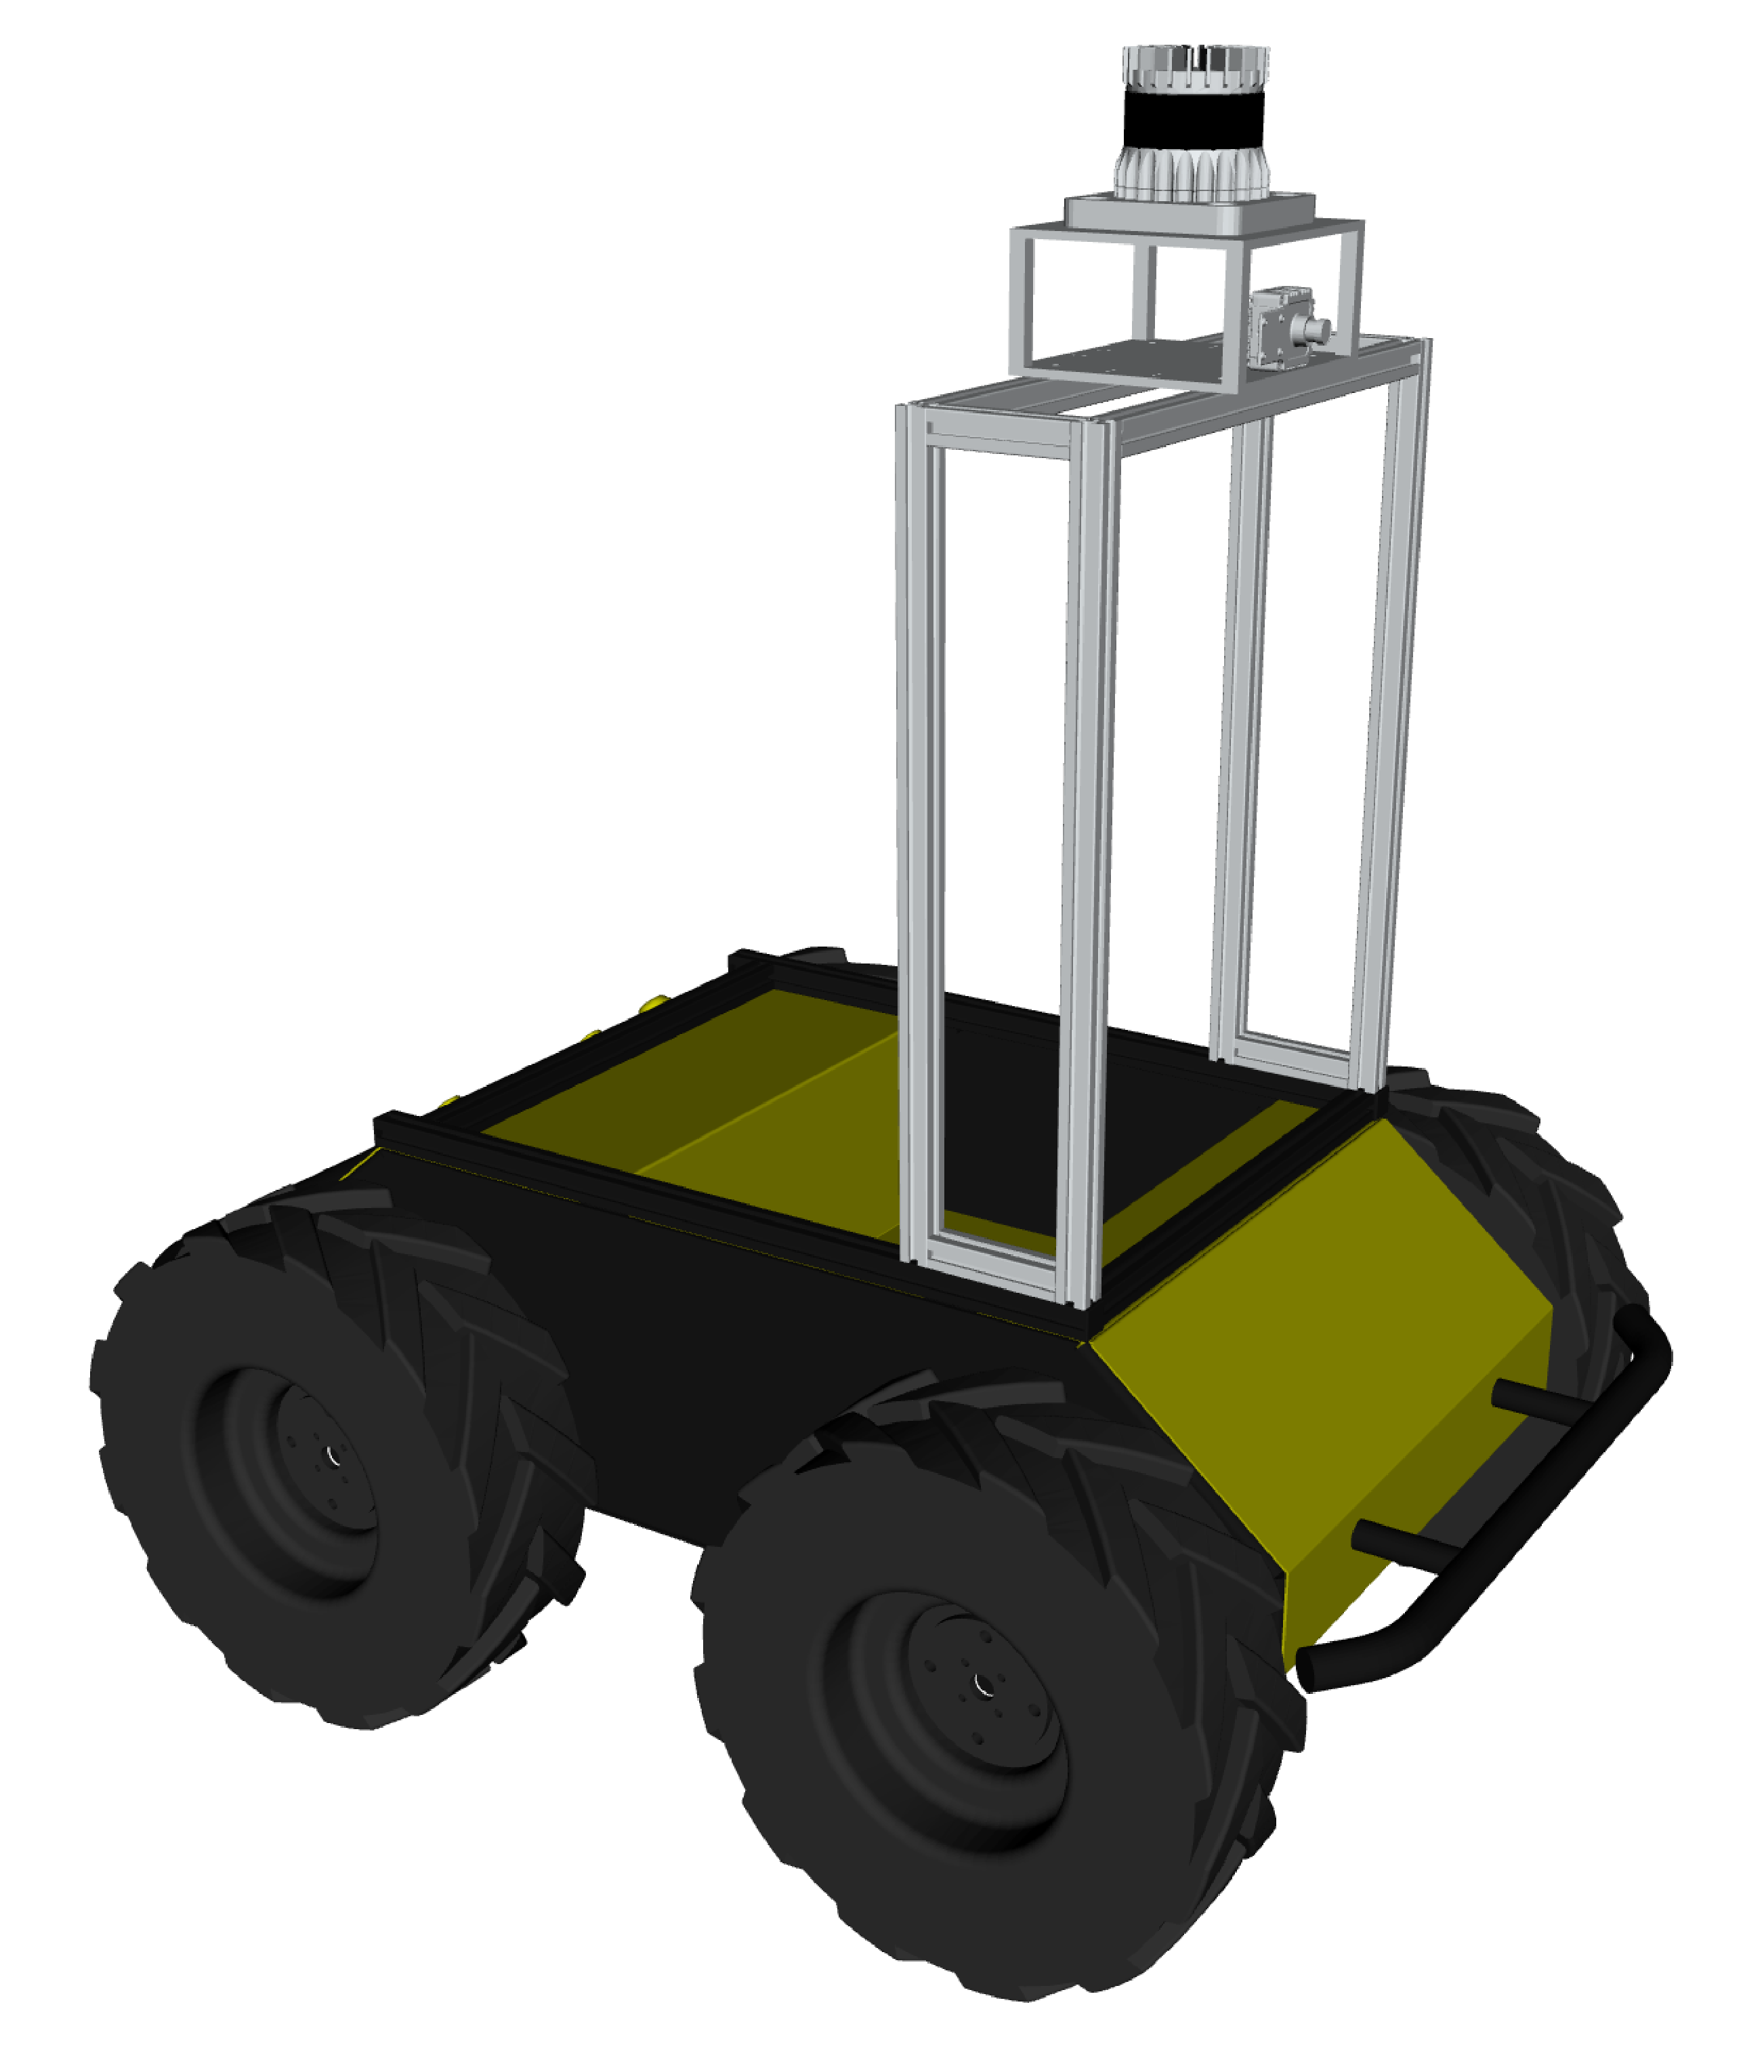
\includegraphics[width = 0.5\textwidth]{Figures/figHuskyRviz.pdf}
  \caption{Rviz2 visualisation of mobile robot running in ROS 2. This acts as a digital twin corresponding to the physical robot.}
  \label{fig:M:AN:MC:digitalTwin}
\end{figure}

\FloatBarrier
\subsubsection{Simulation Setup}
Simulation of the robotic system is run in ROS 2 Galactic Geochelone, by launching \lstinline{sim_husy.launch.py}. This brings up the mobile robot in a Gazebo simulation including a LiDAR simulation. Figure \ref{fig:R:CMR:gazeboSim} illustrates the mobile robot simulated in Gazebo and its digital twin with the corresponding laser scan visualisation in Rviz2.

\begin{figure}[htp!]
  \centering
  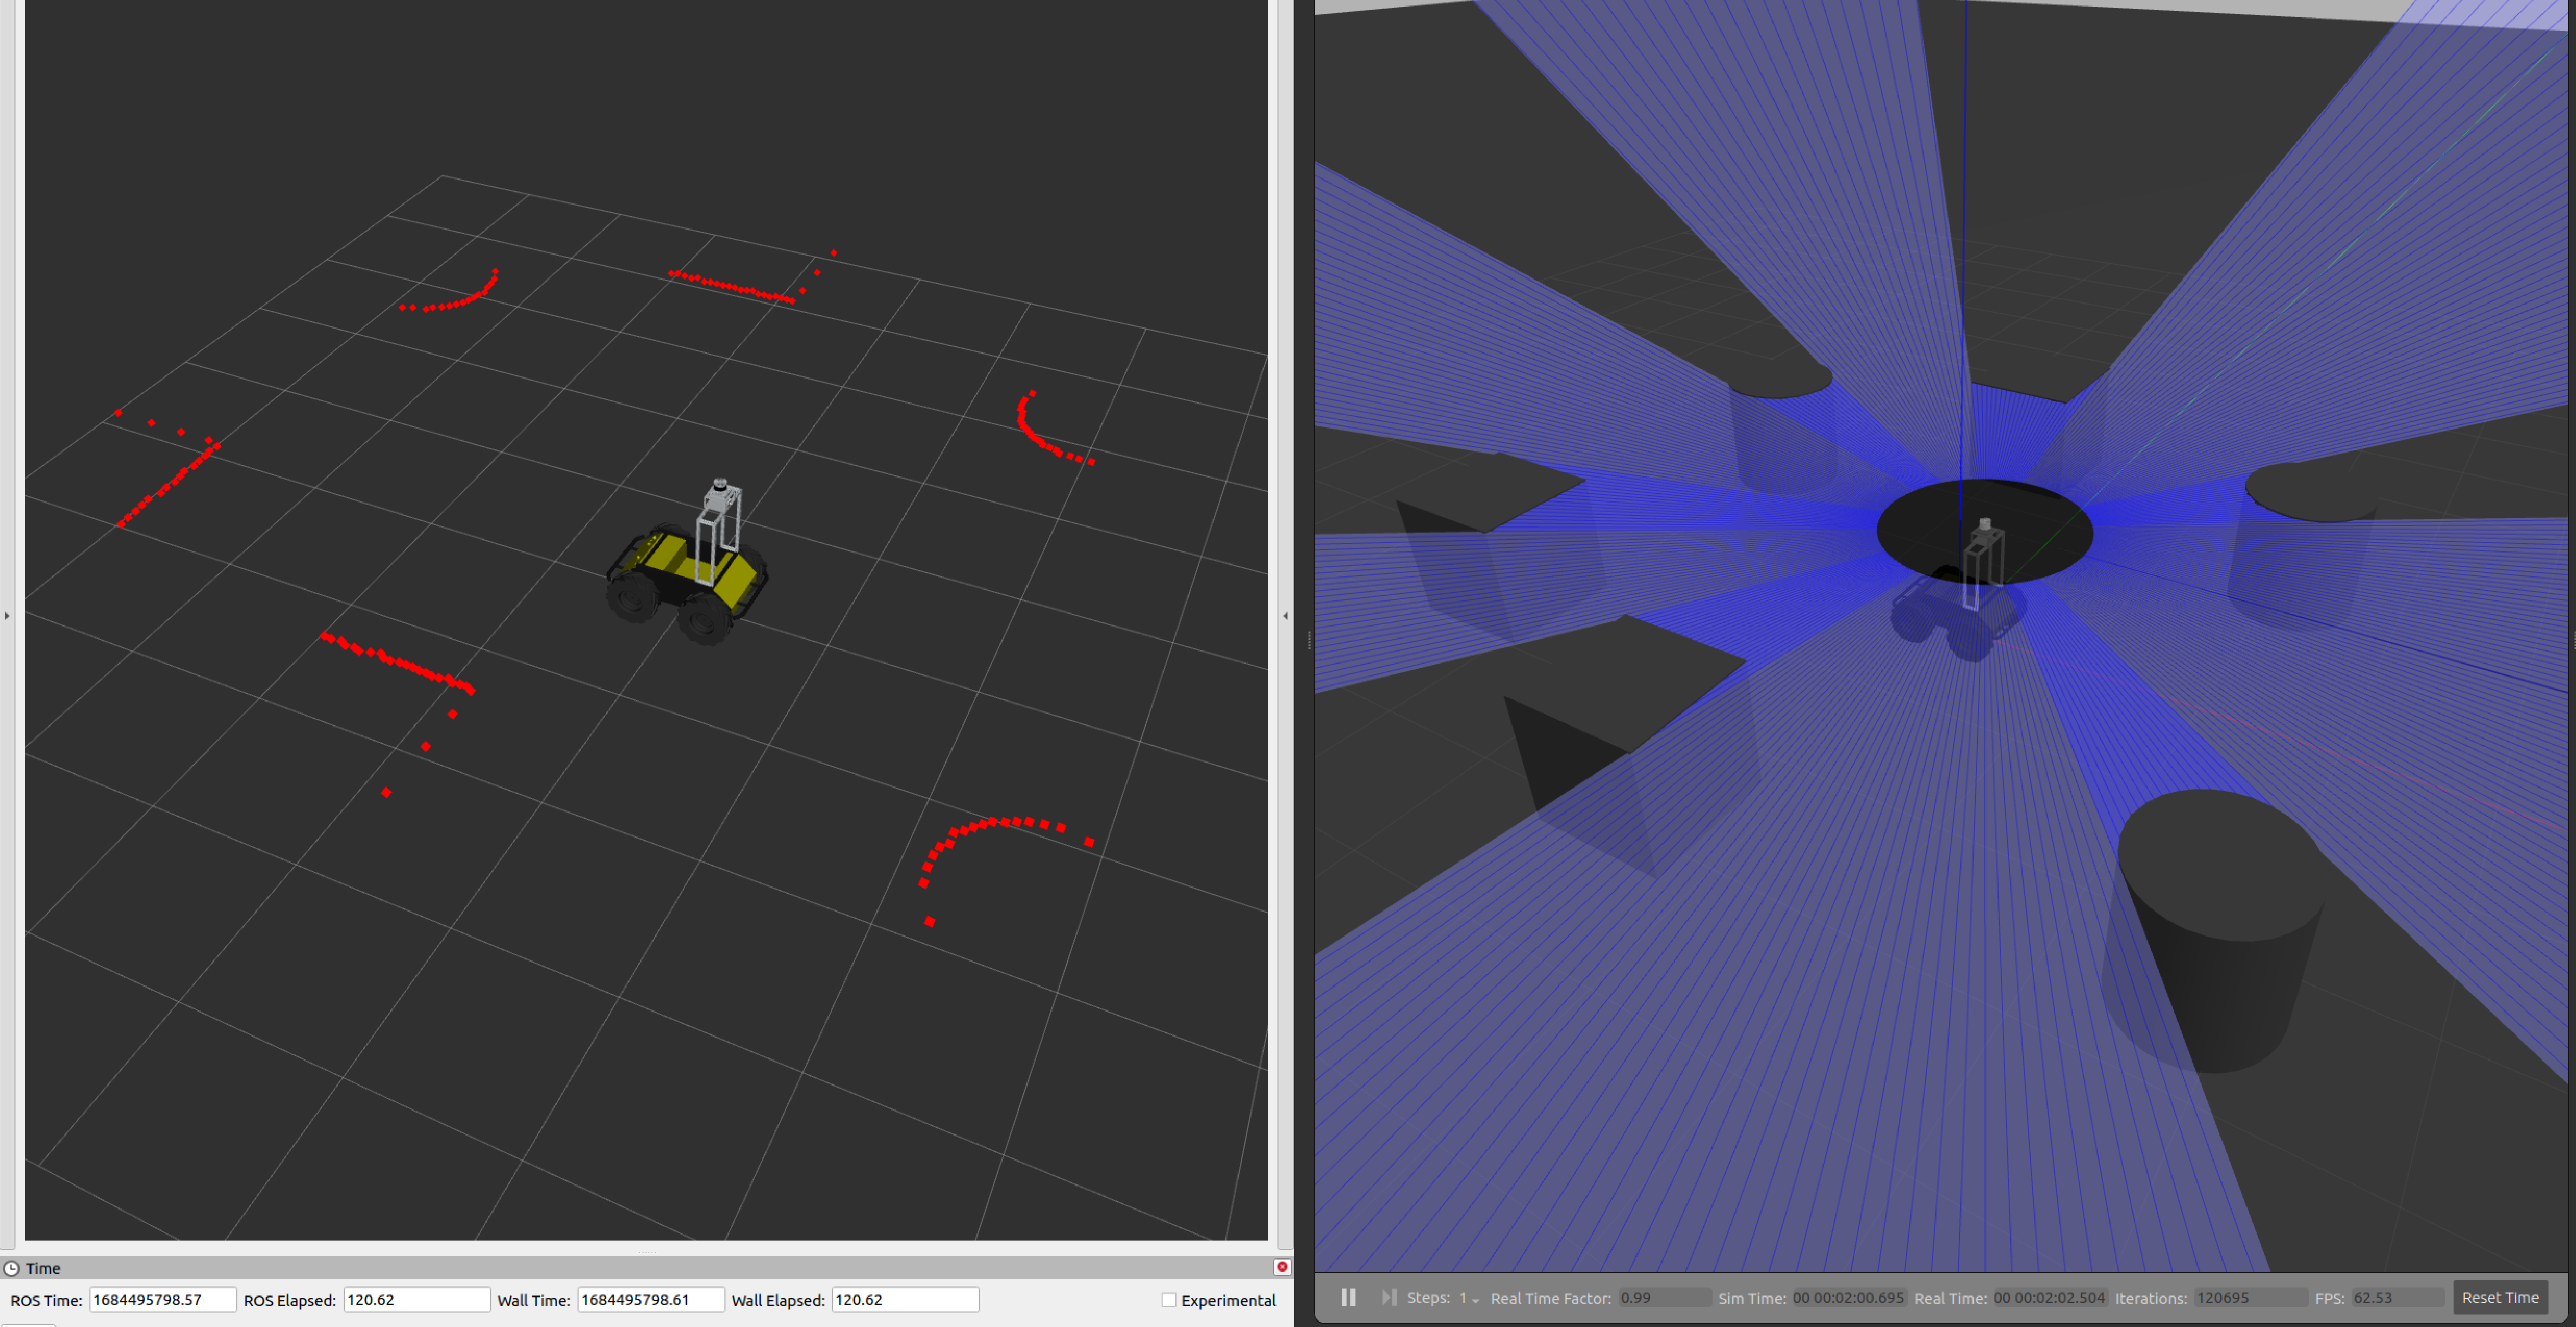
\includegraphics[width = 0.98\textwidth]{Figures/figHuskyGazebo.pdf}
  \caption{Mobile robot simulation running in a Gazebo environment. Corresponding Digital twin and laser scan visualisation can be seen in Rviz2. }
  \label{fig:R:CMR:gazeboSim}
\end{figure}

\FloatBarrier
\subsection{Simultaneous Localisation and Mapping}\label{sec:R:AN:SLAM}

\FloatBarrier
\subsubsection{Physical Experiment}
Physical testing of SLAM performance was done at UiA Campus Grimstad. First mobile robot was launched using \lstinline{husky_launch.py} from the custom ROS 2 package \lstinline{husky_group}. Then SLAM toolbox was launched in online asynchronous mapping with default parameters. NAV 2 is used along with SLAM toolbox to move the mobile robot through the lab. This would generate a map while travelling from the machine lab at campus to the elevators, this is a distance of about \textbf{DISTANCE}, and an area of about \textbf{AREA}. The resulting map can be seen in figure \ref{fig:R:AN:SLAM:figUiaMap}.

\begin{figure}[htp!]
  \centering
  \includesvg[angle=90, width = 0.5\textwidth]{Figures/figUiaMap.svg}
  \caption{Map of Machine Lab and Corridor at UiA Campus Grimstad. The map has been generated through SLAM with an autonomous mobile robot.}
  \label{fig:R:AN:SLAM:figUiaMap}
\end{figure}

\FloatBarrier
\subsubsection{Simulation Experiment}
Performance of SLAM in a simulation environment was tested by launching the mobile robot simulation using \lstinline{sim_husky.launch.py} from the custom ROS 2 package \lstinline{husky_group}. Then a simple environment was created in Gazebo. SLAM Toolbox was then launched in online asynchronous mapping with parameters provided in \lstinline{husky_group} (\lstinline{mapper_params_online_async.yaml}). The mobile robot simulation was then driven around in this Gazebo environment. Figure \ref{fig:R:H:SLAM:figSLAMSim} illustrates the Gazebo test environment along with the corresponding map generated by SLAM.

\begin{figure}[htp!]
  \centering
  \begin{minipage}[b]{0.49\textwidth}
        \centering
        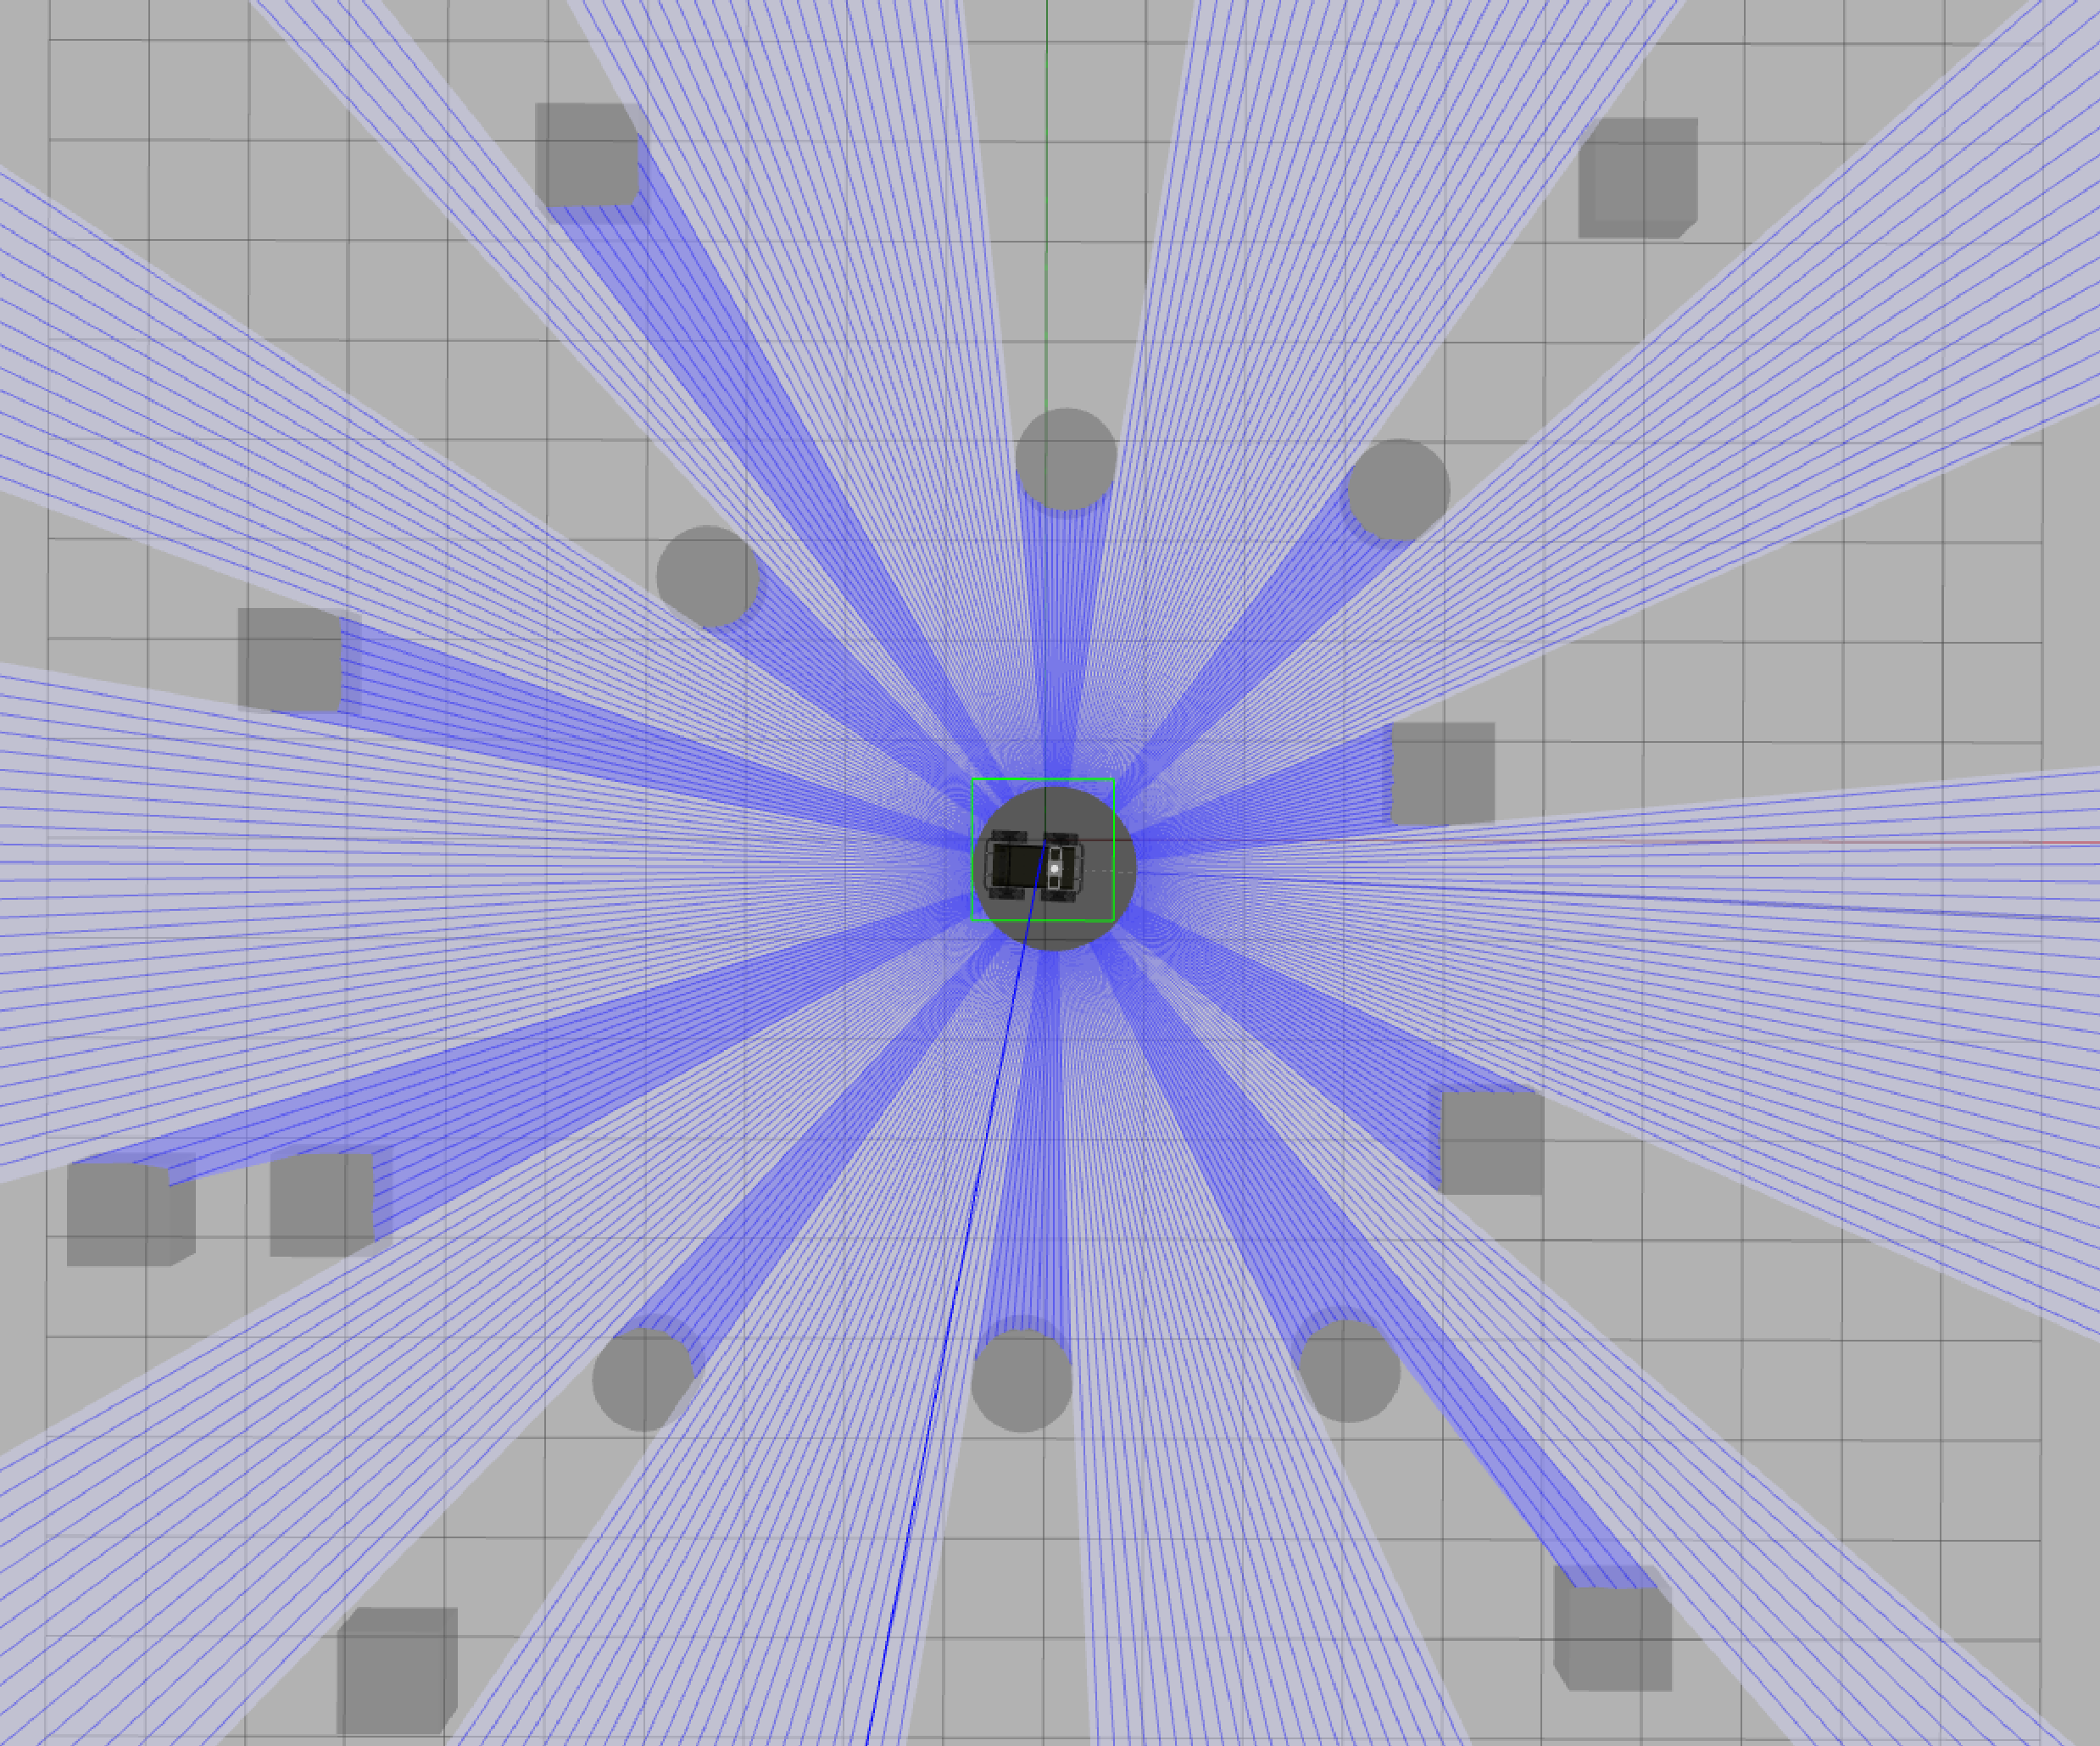
\includegraphics[width = 0.9\textwidth]{Figures/figMapGazeboSim2.pdf}
  \end{minipage}
  \hfill
  \begin{minipage}[b]{0.49\textwidth}
    \centering
    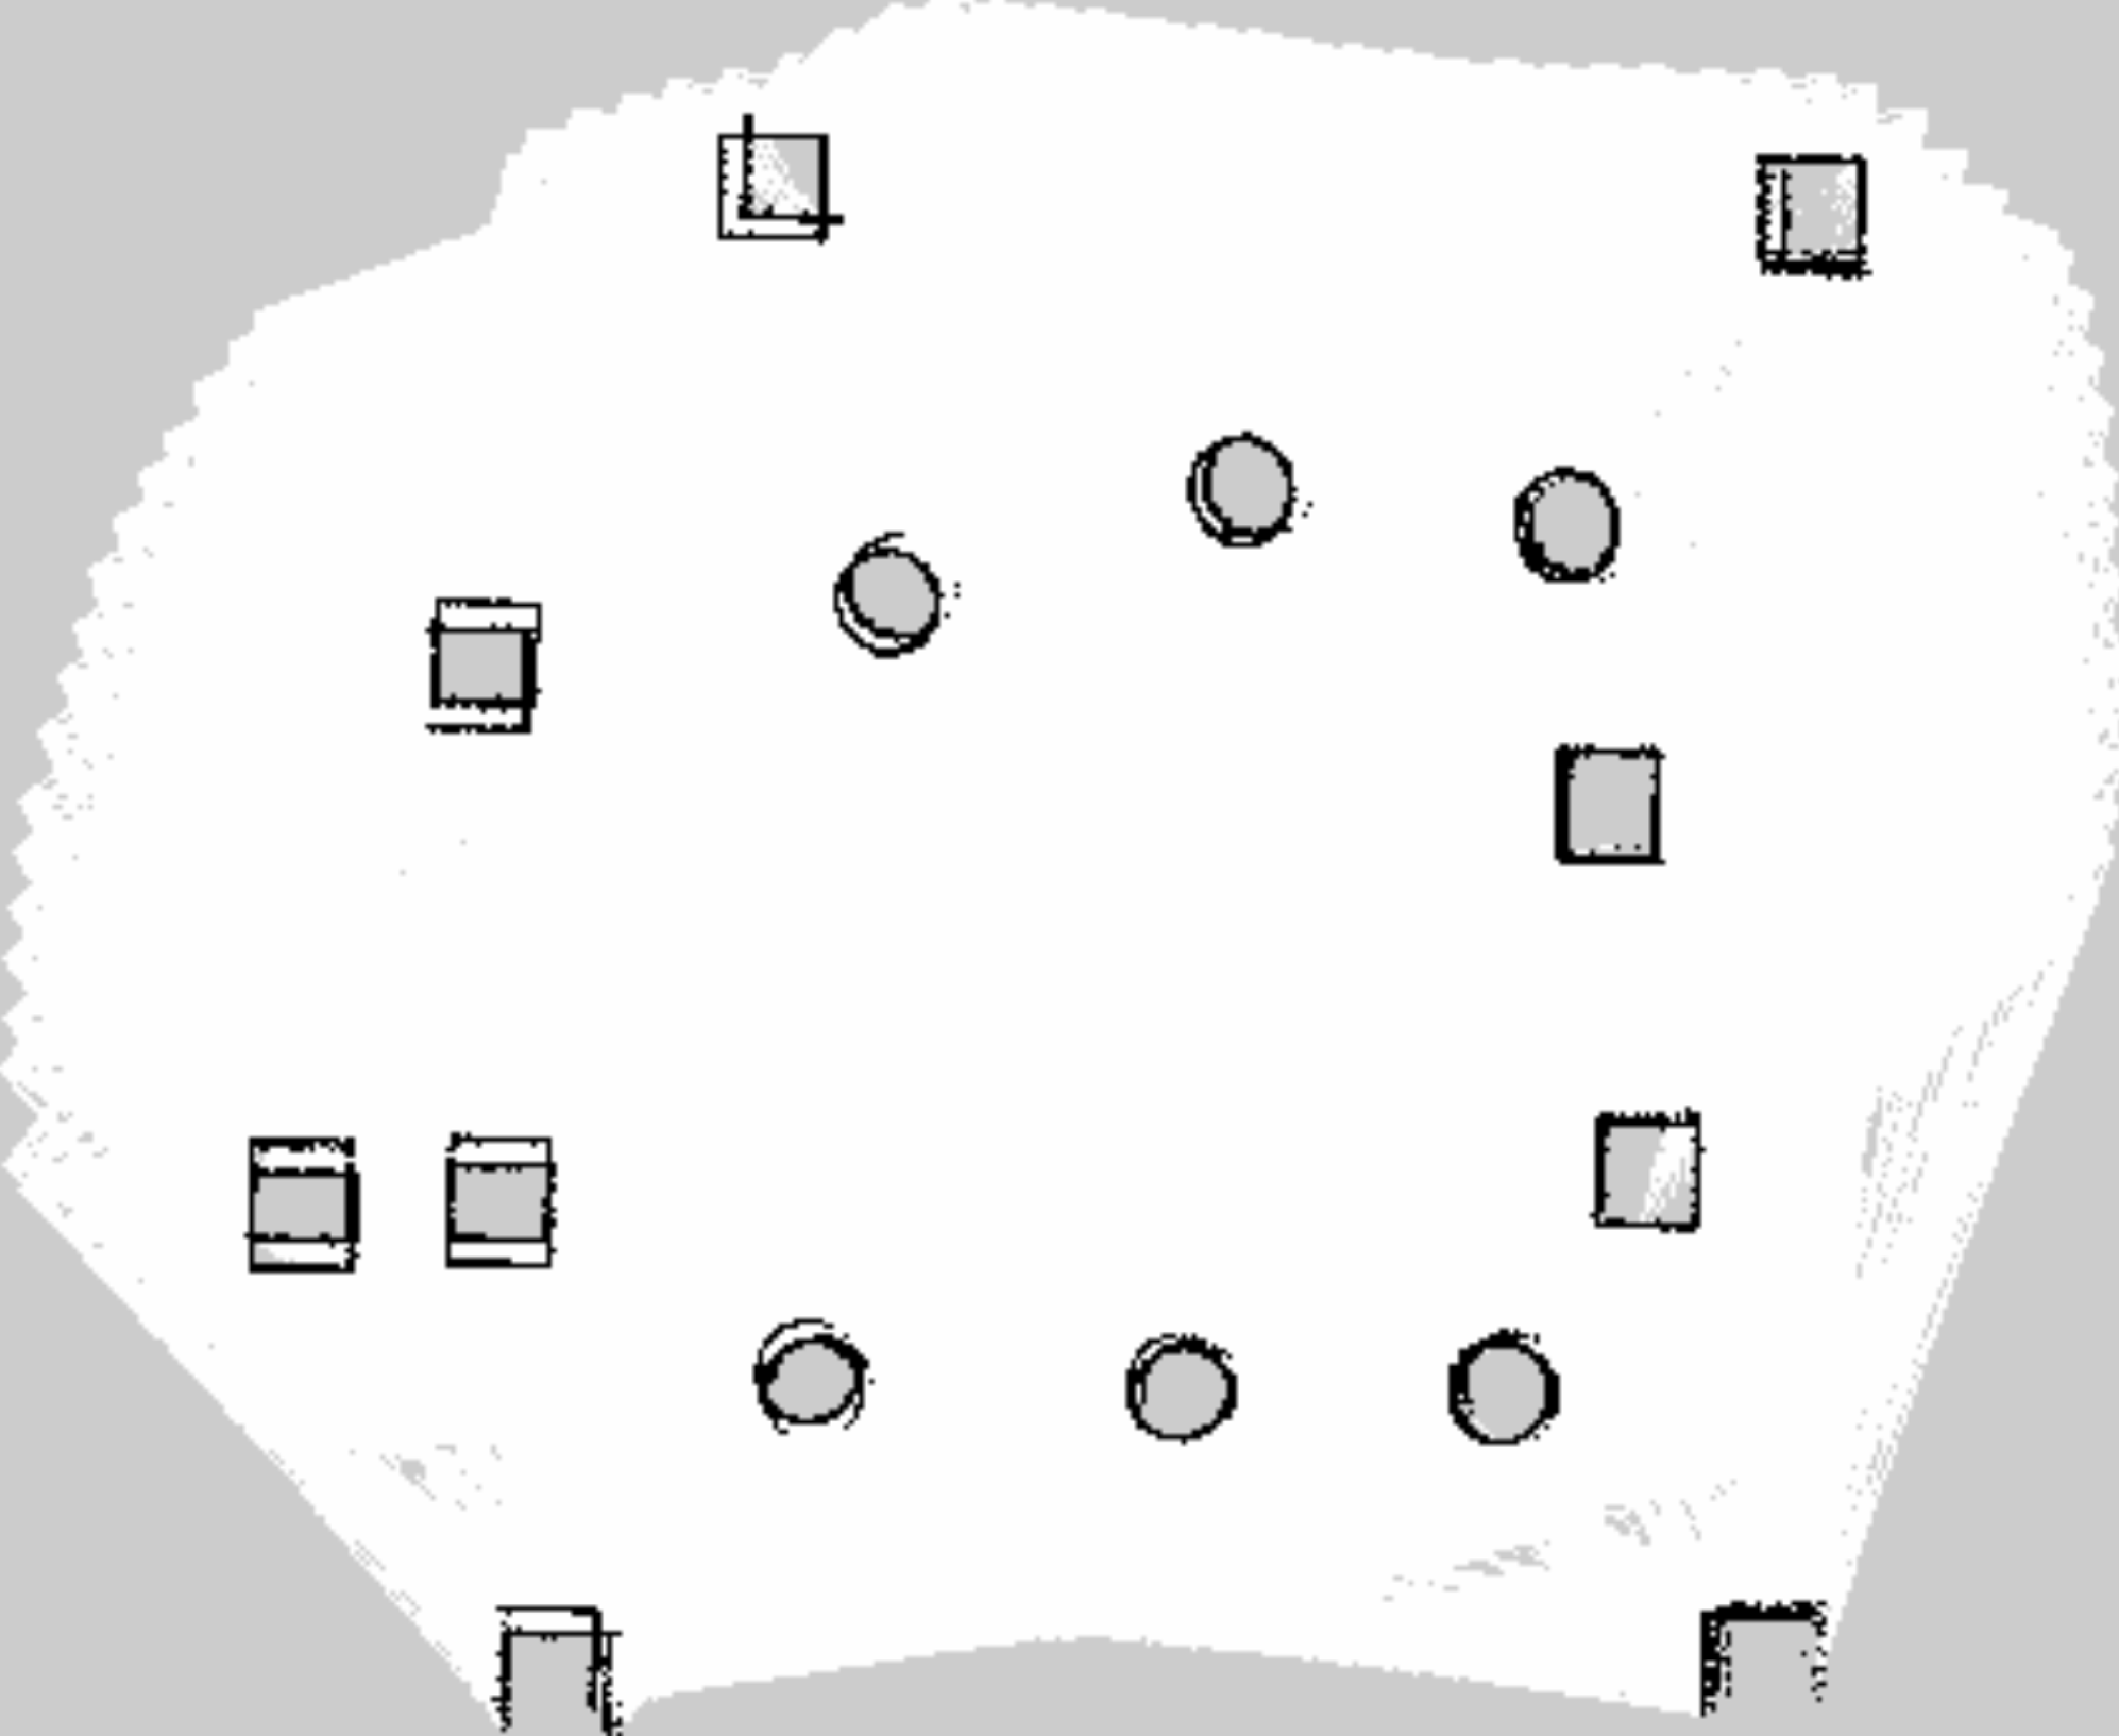
\includegraphics[width = 0.9\textwidth]{Figures/figMapSim.pdf}
  \end{minipage}
  \caption{SLAM testing in Gazebo simulation environment. \textbf{Left:} Gazebo test environment with mobile robot. Laser scan is visualised. \textbf{Right:} SLAM map generated during test in Gazebo test environment.}
  \label{fig:R:H:SLAM:figSLAMSim}
\end{figure}

\FloatBarrier
\subsection{Navigation}\label{sec:R:AN:Navigation}
\FloatBarrier
\subsubsection{Physical Experiment}
Navigation was tested by running the complete setup, together with SLAM, as mentioned in section \ref{sec:R:AN:SLAM}. As the map was generated on-the go, goal poses were manually updated by the operator as the map continued to be updated. Figure \ref{fig:R:H:SLAM:figNavUia} illustrates how the autonomous navigation is visualised on the operators computer using Rviz2.

\begin{figure}[htp!]
  \centering
  \begin{minipage}[b]{0.49\textwidth}
        \centering
        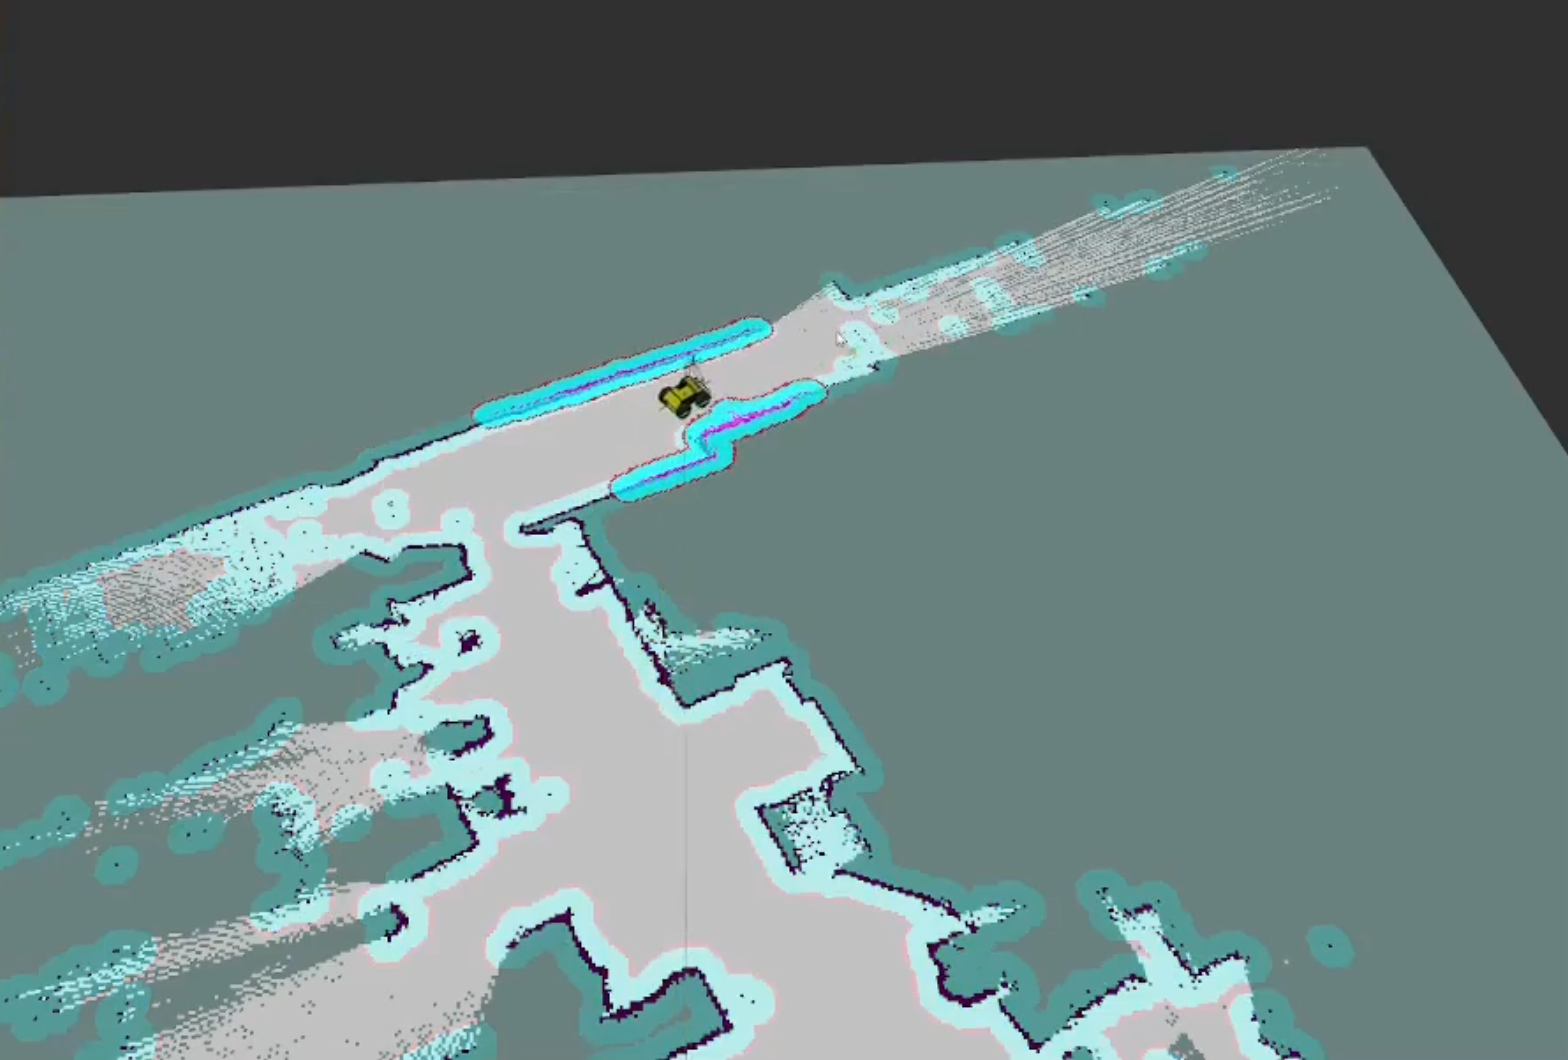
\includegraphics[width = 0.98\textwidth]{Figures/figNavUia2.png}
  \end{minipage}
  \hfill
  \begin{minipage}[b]{0.49\textwidth}
    \centering
    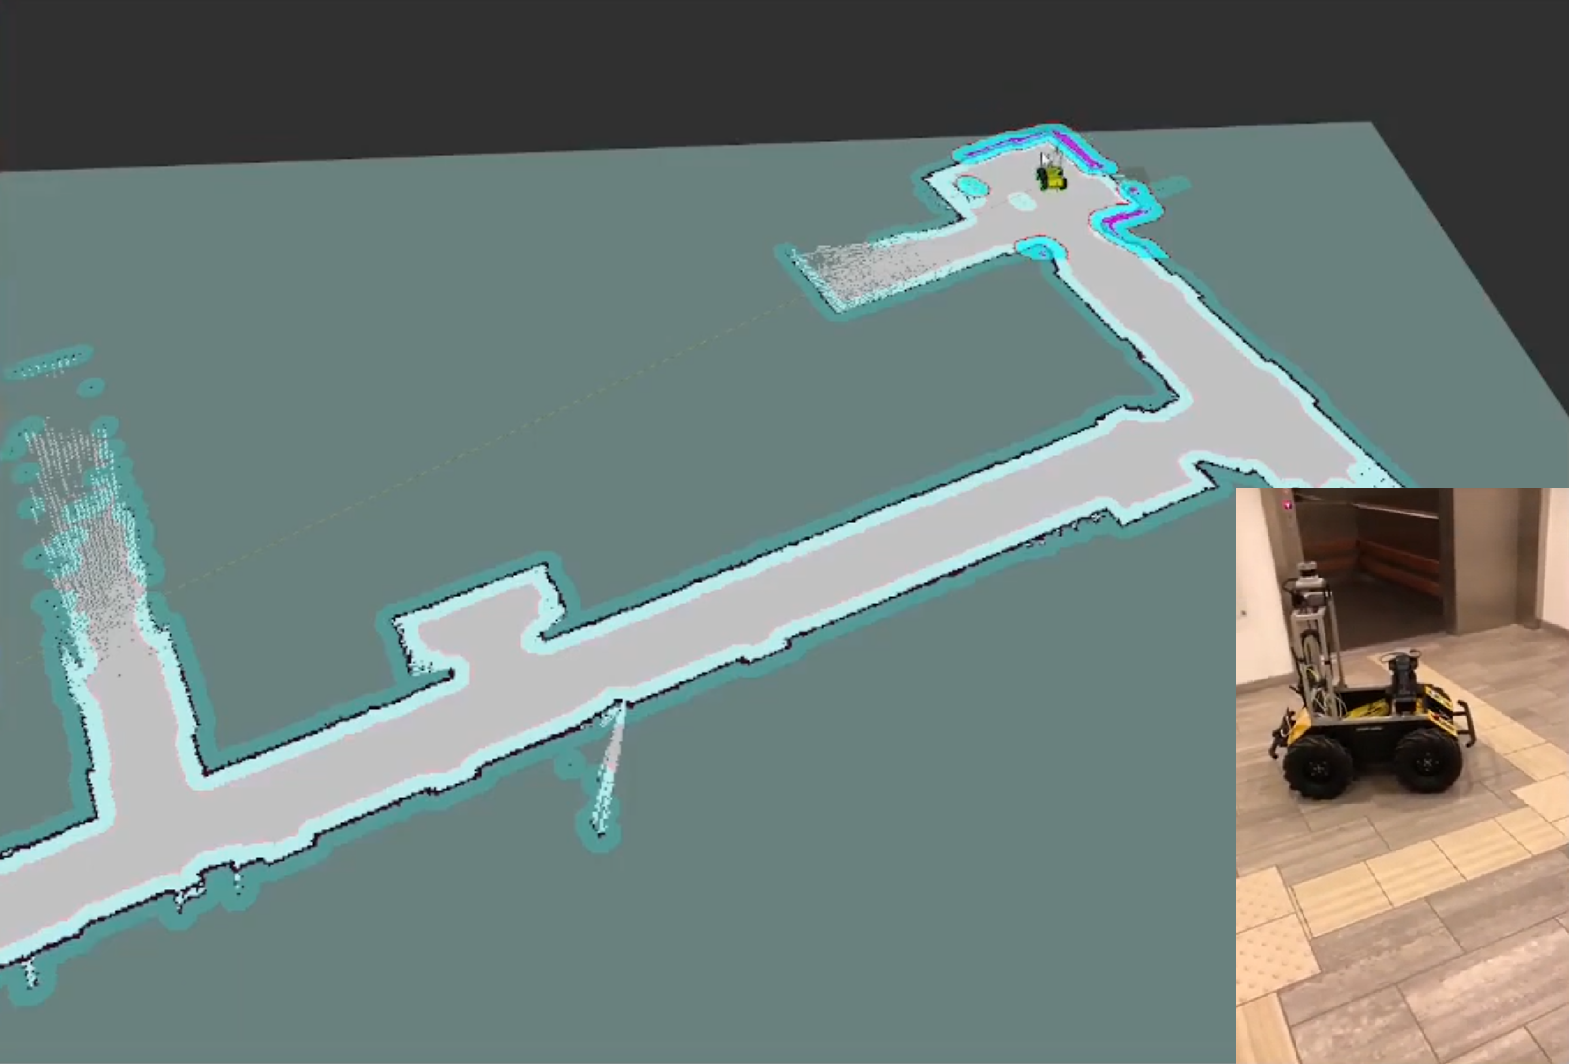
\includegraphics[width = 0.98\textwidth]{Figures/figNavUia4.png}
  \end{minipage}
  \caption{Mobile robot Running NAV2 along with SLAM on ROS2. This is a visualisation of Rviz2 where the mobile robot is illustrated as a 3D model on top of the generated map.}
  \label{fig:R:H:SLAM:figNavUia}
\end{figure}

During navigation testing, collision avoidance was tested by placing a person in front of the robot. Figure \ref{fig:R:AN:N:CA:CollisionAvoidance1} and \ref{fig:R:AN:N:CA:collisionAvoidance2} illustrates this test. In figure \ref{fig:R:AN:N:CA:CollisionAvoidance1} the robot is not close enough to see the pedestrian in its rolling window (pink overlay). A few moments later, a pedestrian has appeared in the rolling window. The resulting trajectory can be seen as the green line in figure \ref{fig:R:AN:N:CA:collisionAvoidance2}.

\begin{figure}[htp!]
  \centering
  \begin{minipage}[b]{0.49\textwidth}
  \centering
    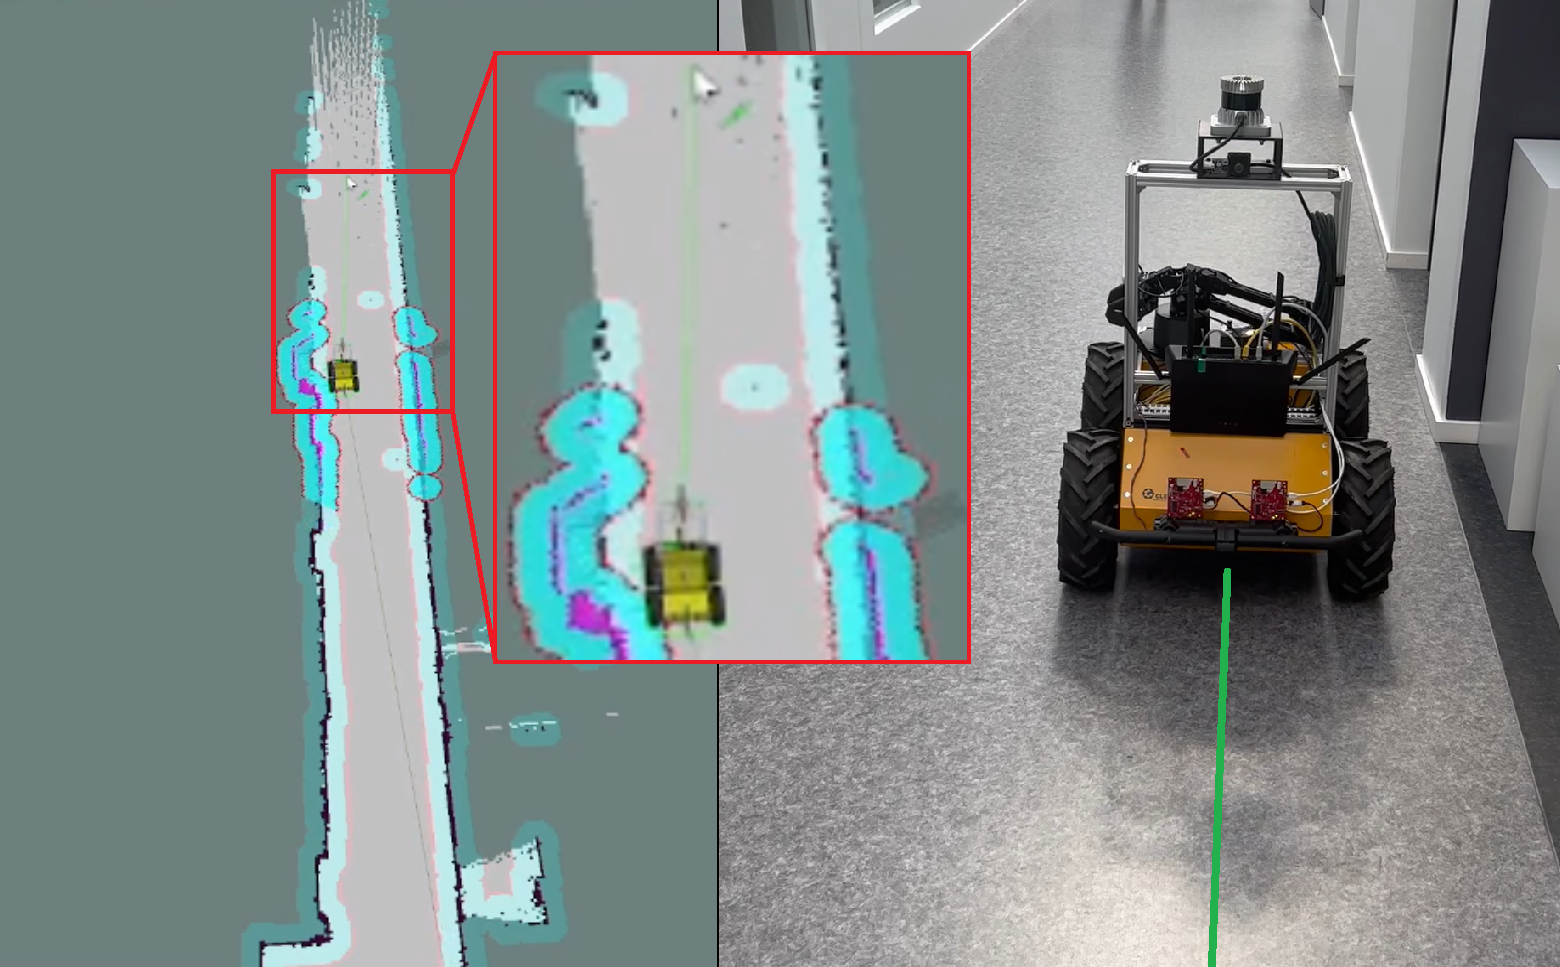
\includegraphics[width = 0.98\textwidth]{Figures/figuiaCollisionAvoidMerged1.png}
    \caption{Robot navigating through a hallway. The robot is not close enough to the camera-man to noctice him in the rolling window. Notice how the trajectory (green line) goes straight forward through the camera-man.}
    \label{fig:R:AN:N:CA:CollisionAvoidance1}
  \end{minipage}
  \hfill
  \begin{minipage}[b]{0.49\textwidth}
    \centering
    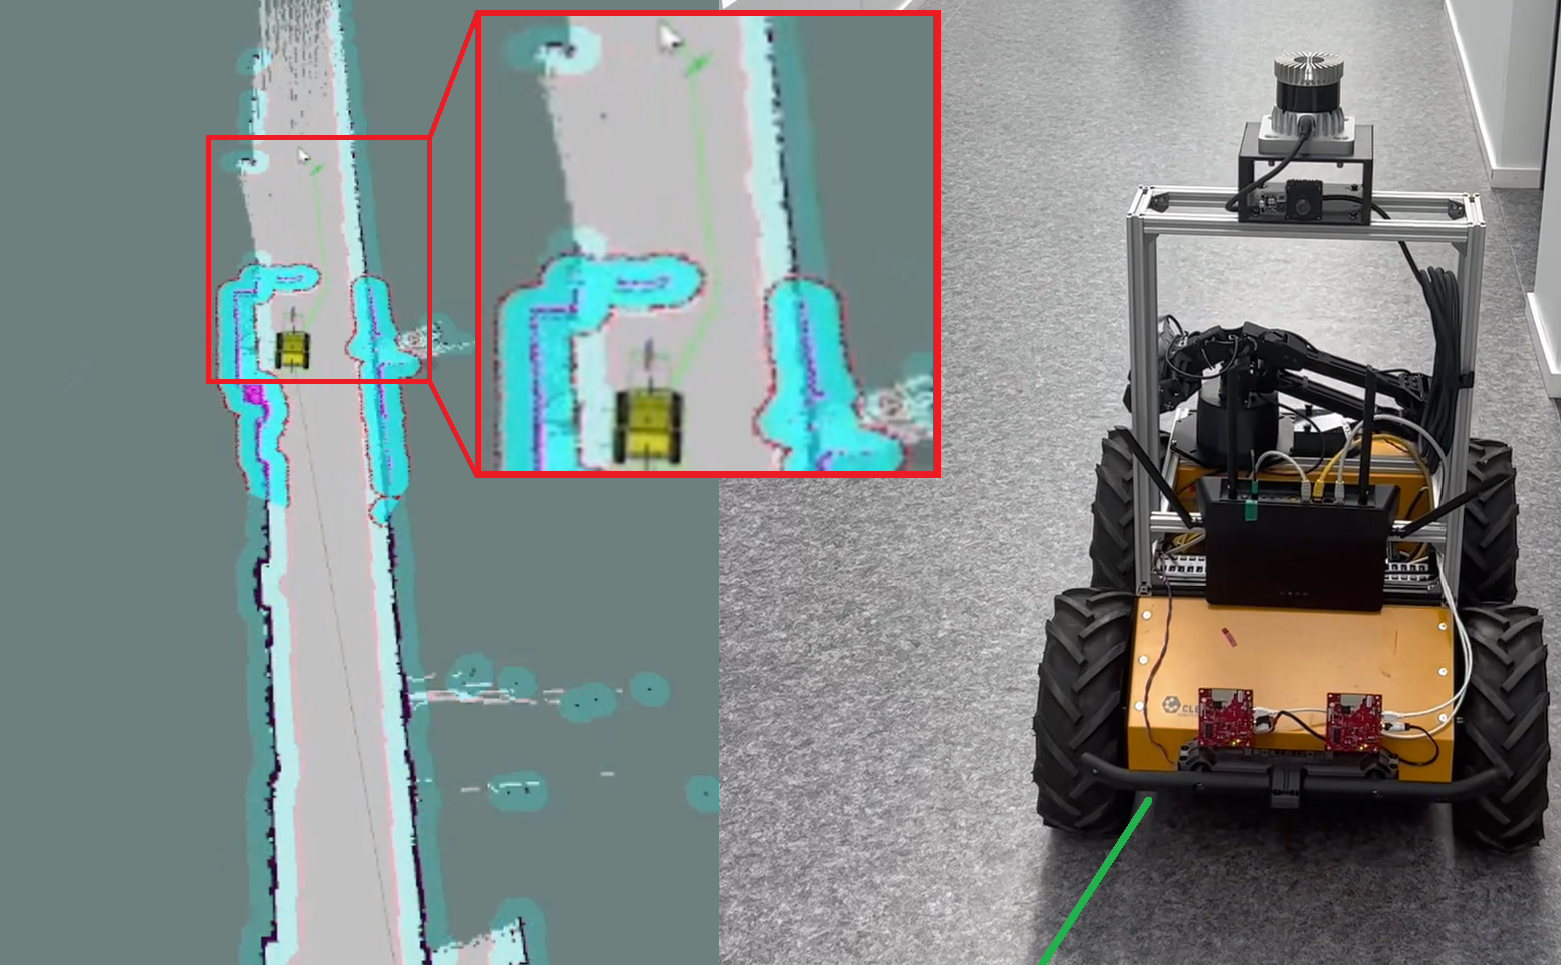
\includegraphics[width = 0.98\textwidth]{Figures/figuiaCollisionAvoidMerged2.png}
    \caption{Robot navigating around obstacle. In this figure, the camera-man can be seen in front of the robot in the rolling window. Notice how the trajectory (green line) goes around the object.}
    \label{fig:R:AN:N:CA:collisionAvoidance2}
  \end{minipage}
\end{figure}

\FloatBarrier
\subsubsection{Simulation Experiment}
Testing of autonomous navigation in a simulation environment was done in a similar way as SLAM simulation testing. First, the mobile robot simulation is launched using \lstinline{sim_husky.launch.py} from the custom ROS 2 package \lstinline{husky_group}. Then, a simple Gazebo environment is created by placing shapes around the mobile robot. SLAM is then launched in online asynchronous mode with parameters provided by \lstinline{husky_group} (\lstinline{mapper_params_online_async.yaml}). The mobile robot is moved around the environment to construct a map. Finally, NAV 2 navigation is launched with parameters provided by \lstinline{husky_group}, and goal poses are set. Figure \ref{fig:R:H:NAV:figNav2Sim} illustrates gazebo test environment along with a map and navigational visualisation in Rviz2.

\begin{figure}[htp!]
  \centering
  \begin{minipage}[b]{0.49\textwidth}
        \centering
        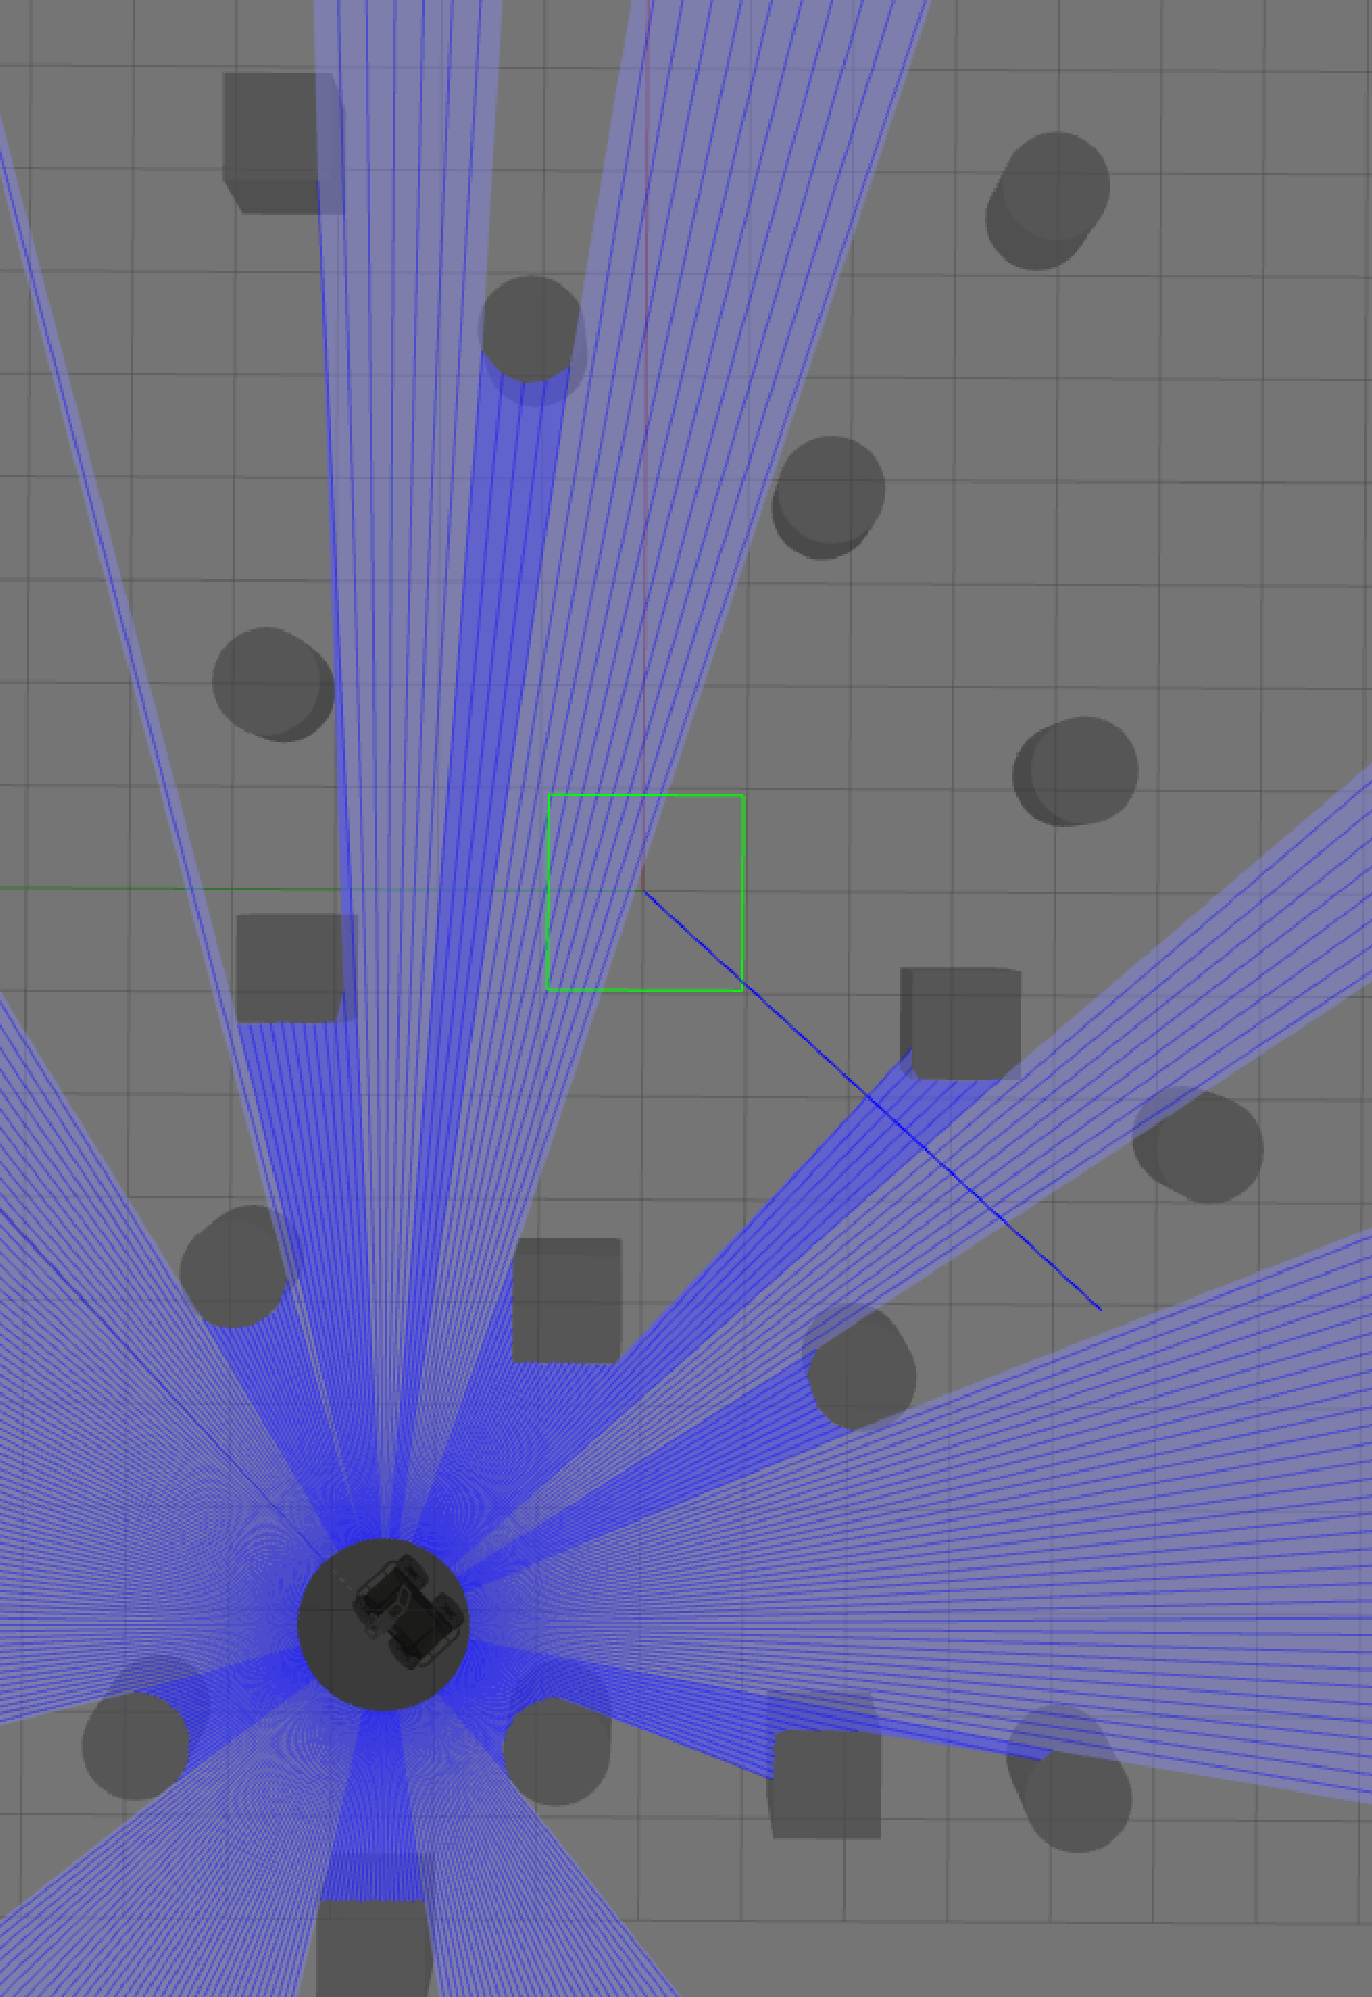
\includegraphics[width = 0.7\textwidth]{Figures/figNav2GazeboSim2.pdf}
  \end{minipage}
  \hfill
  \begin{minipage}[b]{0.49\textwidth}
    \centering
    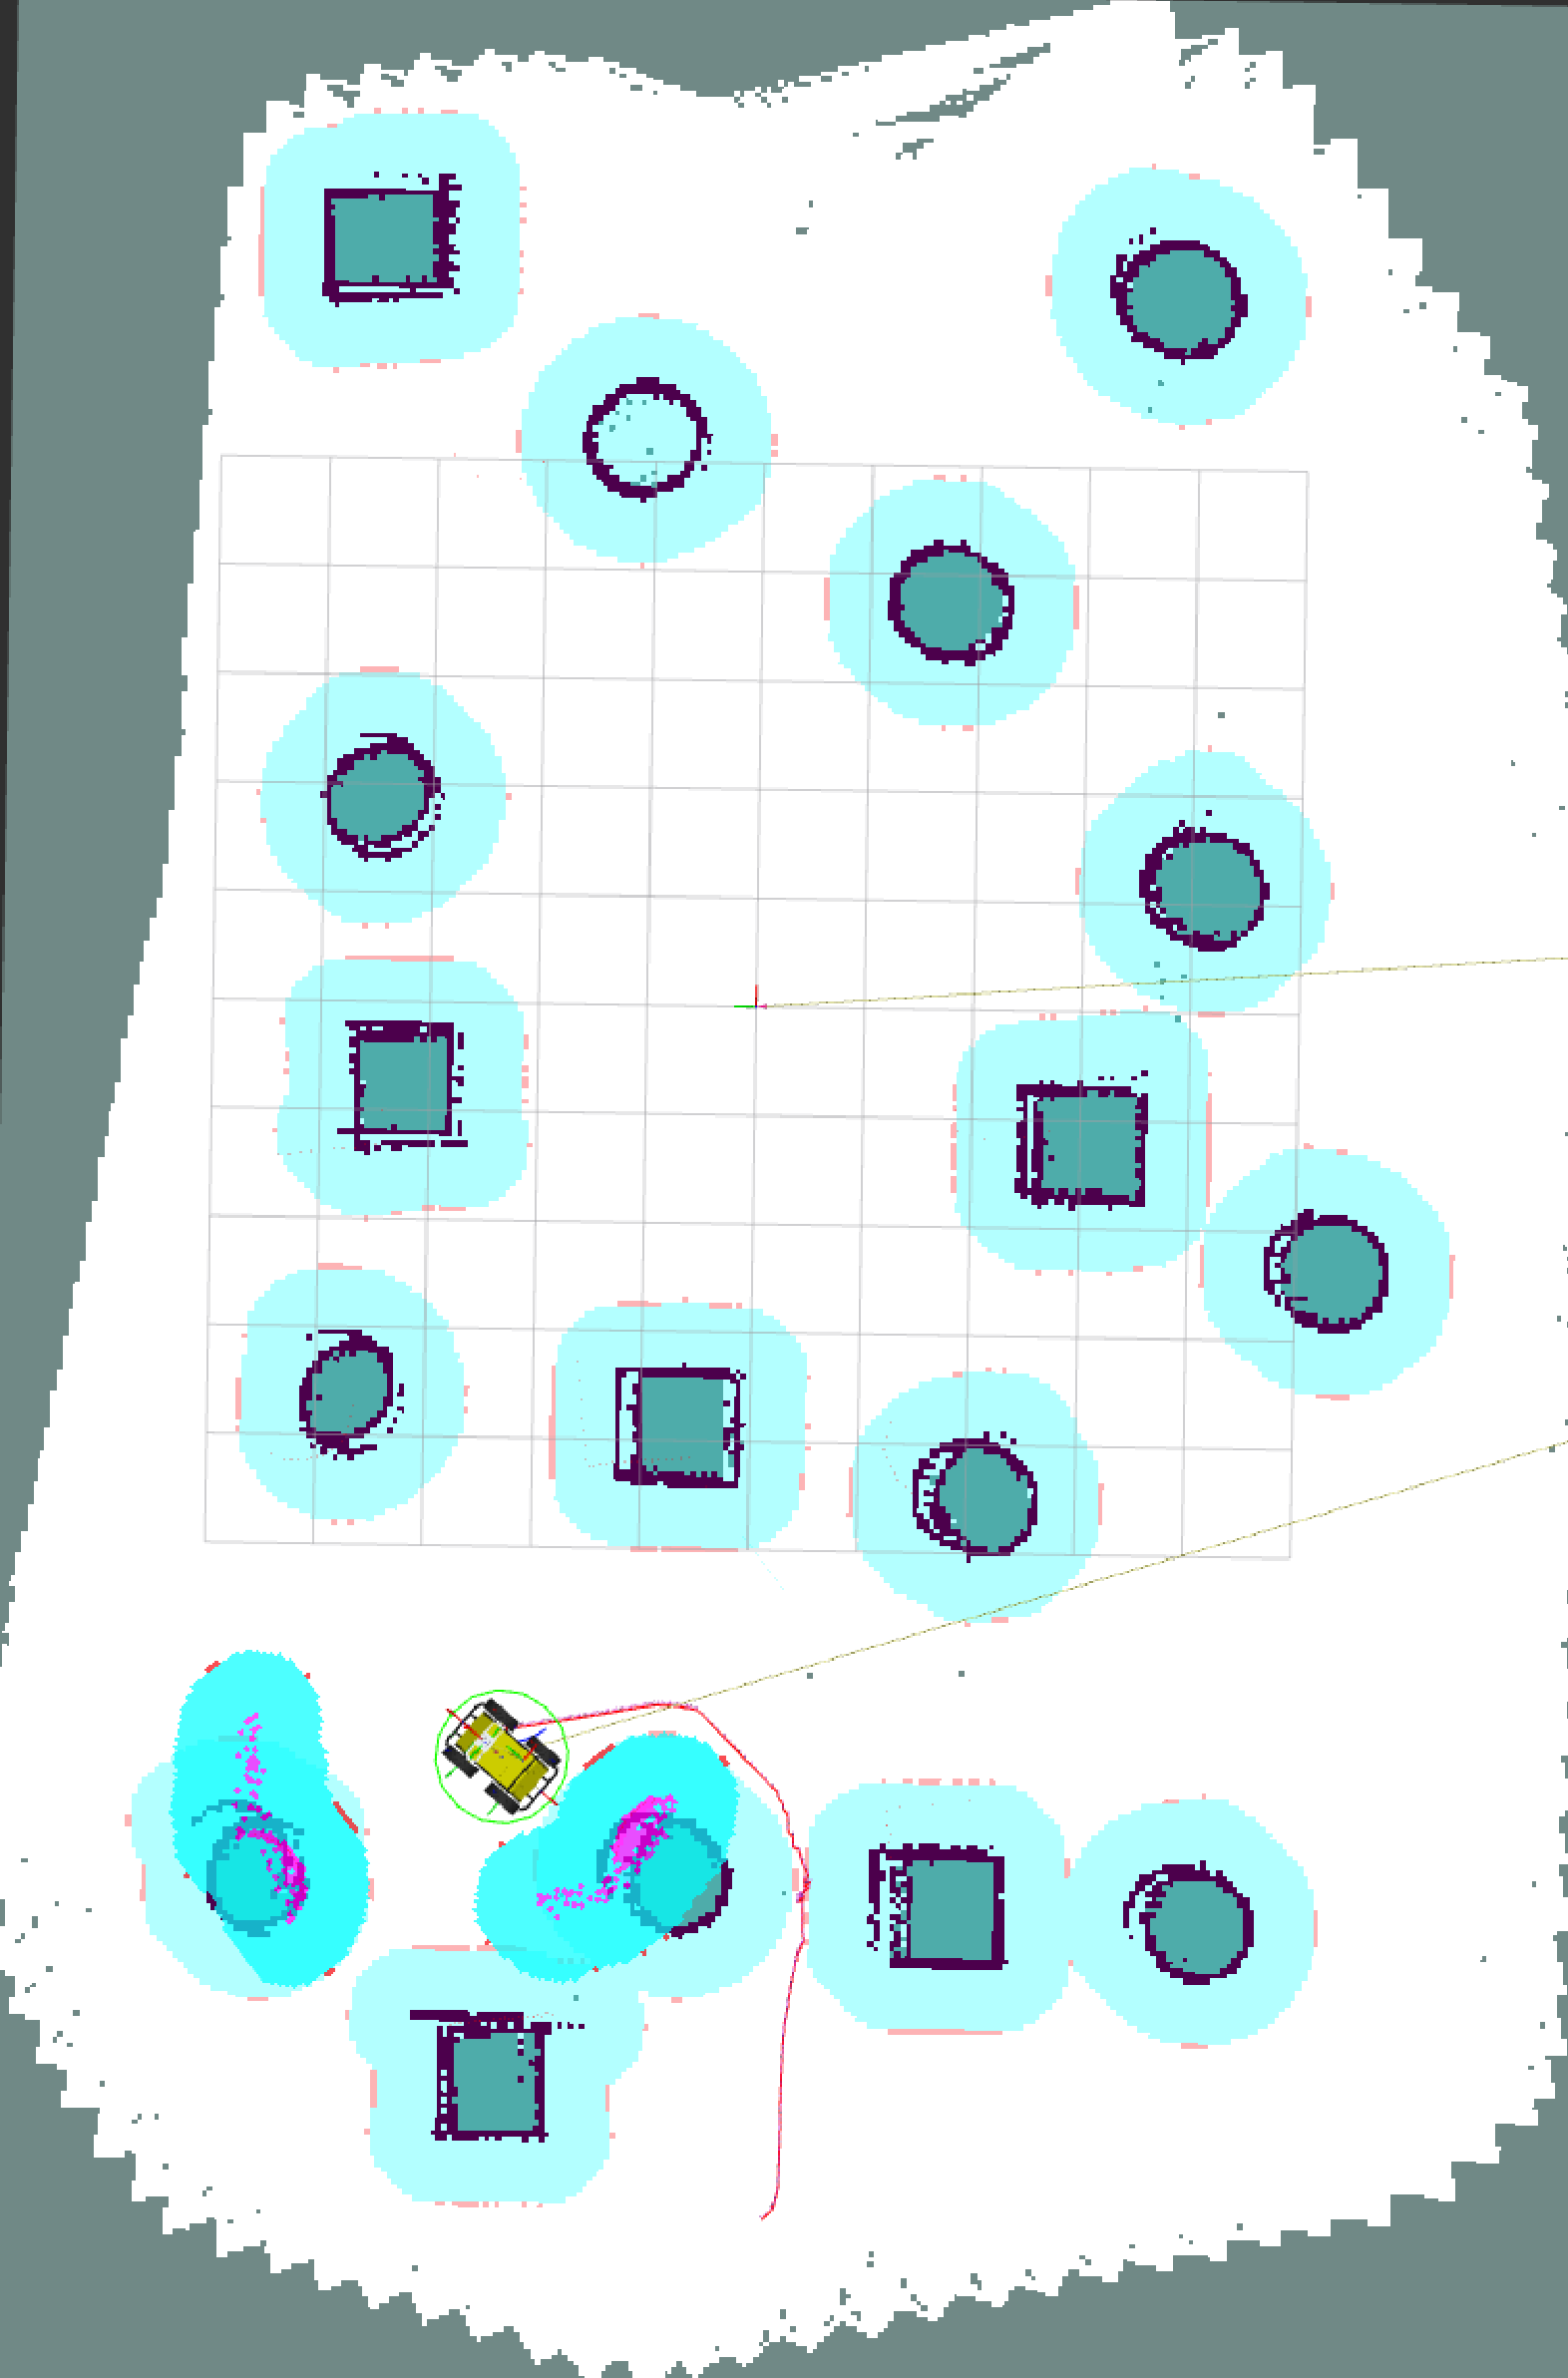
\includegraphics[width = 0.67\textwidth]{Figures/figNav2MapSim2.pdf}
  \end{minipage}
  \caption{NAV 2 testing in simple Gazebo environment. \textbf{Left:} Gazebo simulation test environment with mobile robot. \textbf{Right:} Rviz 2 visualisation of mobile robot moving around in the map constructed from this environment. Red line illustrates planned trajectory.}
  \label{fig:R:H:NAV:figNav2Sim}
\end{figure}

%\section{Pick and Place} \label{sec:R:PickAndPlace}
% Pick and place operations is achieved through a combination of three systems. The first system is the VX300 manipulator itself and it's ROS2 Moveit2 packages described in section \ref{sec:M:MRC:Manipulator}. The second system is the computer vision system described in section \ref{sec:M:MRC:MachineVision}. This includes the vision camera, its drivers and the AprilTag based object detection system. The last system needed is the custom pick and place ROS2 package described in section \ref{sec:M:A:HuskyPickAndPlace}. Results regarding object detection and the custom pick and place ROS2 package will be presented.



% \subsection{Custom ROS2 Packages}
% The custom ROS2 packages has been built and tested around a specific robotic system. It is not likely that it will work for other types of robotic systems out of the box. 

\FloatBarrier
\section{Custom Pick and Place Bring-Up Package}
 The custom mobile ROS 2 package \lstinline{husky_interbotix} described in section \ref{sec:M:PAP:CutsomPAPBringup} is used to bring up the complete pick and place system. As mentioned in section \ref{sec:M:PAP:CutsomPAPBringup} this package can be used with the physical system on the "Manipulator Xavier" as well as a virtual robot for simulation. Figure \ref{fig:R:P&P:CSP:scenePublisher1} illustrates the manipulators visualisation in Rviz 2 with the vision camera mounted to the gripper. Figure \ref{fig:R:P&P:CSP:scenePublisher2} illustrates the collision boxes published to the planning scene by the custom scene geometry publisher (described in method section \ref{sec:M:PAP:SceneGeometryPublisher}) upon launch.

\begin{figure}[htp!]
  \centering
  \begin{minipage}[b]{0.49\textwidth}
        \centering
        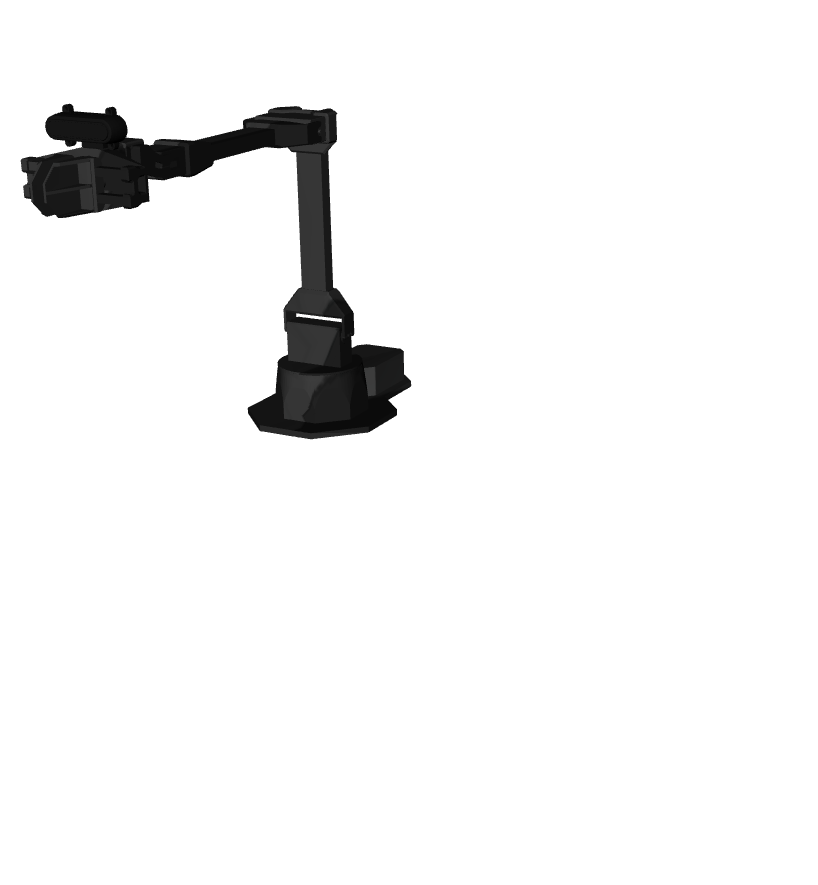
\includegraphics[width = 0.9\textwidth]{Figures/figScenePublisher1.png}
        \caption{Manipulator initiated with Moveit2 and visualised in Rviz2.}
        \label{fig:R:P&P:CSP:scenePublisher1}
  \end{minipage}
  \hfill
  \begin{minipage}[b]{0.49\textwidth}
    \centering
    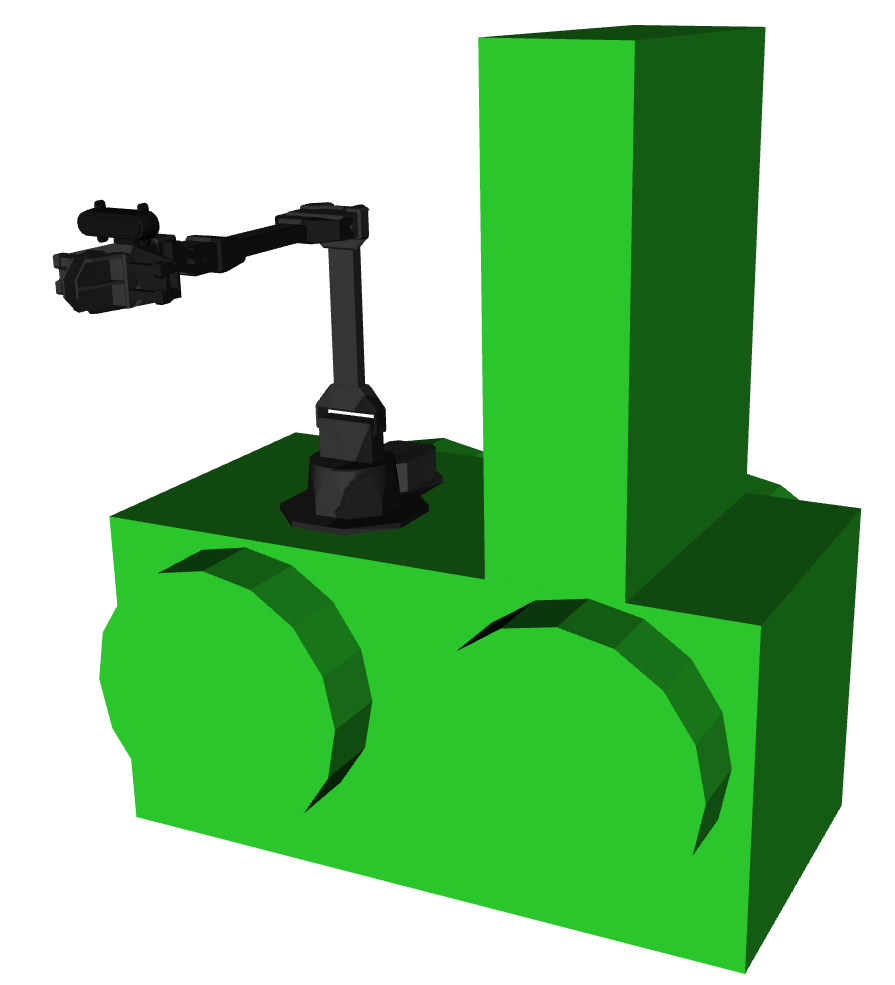
\includegraphics[width = 0.86\textwidth]{Figures/figScenePublisher2.png}
    \caption{Manipulator initiated with Moveit2 and visualised in Rviz2. Collision boxes are published to the planning scene using the custom Scene Publisher ROS2 package.}
    \label{fig:R:P&P:CSP:scenePublisher2}
  \end{minipage}
\end{figure}


% \subsubsection{Husky Pick and Place Package}
% A custom ROS2 package has been made to enable control of the manipulator and get feedback about current operation through the ROS2 network's topic system. The design of this package is described in section \ref{sec:M:A:HuskyPickAndPlace}. Testing has been done to tune the robot's move sequences and to verify the robustness of the ROS2 topic based command and feedback system. 

% \textbf{Do some testing and write a bit about it here}

\FloatBarrier
\section{Top Level} \label{sec:R:TopLevel}
% The full warehouse automation pipeline is set up using the custom ROS2 package "Husky Master Node" described in section \ref{sec:M:A:HuskyMasterNode}. Running this node results in the UGV autonomously navigating to a predefined pick location before running the pick operation. The pick operation includes using computer vision to detect and estimate the pose of the object before picking. After picking, the UGV moves to the place location and the place operation is preformed. Finally, the UGV will return to it's starting position. The complete operation where the robot moves to a pick location, picks an object using MV, moves to a place location, places the object and moves back home was performed twice in a row with success.
The top level system has been tested in three different scenarios:
\begin{itemize}
    \item Physical experiment, with the entire mobile robotic system running in a lab at UiA Campus Grimstad
    \item Simulation experiment, with a simulation of the robotic system running in a simple ROS 2 Gazebo simulation environment. The simulation does not include IMUs, EKF or a computer vision System.
    \item TurtleBot3 Simulation experiment, with a TurtleBot3 gazebo simulation and a virtual Interbotix VX300 robotic arm.
\end{itemize}

Number of navigational goal poses and definition of goal poses have been altered between the tests.

\FloatBarrier
\subsection{Physical Experiment}
Physical testing of the complete warehouse automation pipeline has been performed in the machine lab at UiA Campus Grimstad. Prior to launching the "Husky Master Node" (descried in section \ref{sec:M:TopLevel}), the complete autonomous navigation system including SLAM has been brought in the same way as described in section \ref{sec:R:AN:Navigation}. That is, by first launching the mobile robot using the custom mobile robot bring-up package, then launching SLAM and NAV 2. The pick and place system is also brought up an ready to take commands. This is done using the custom pick and place bring-up package. Figure \ref{fig:R:WA:finalExperiment1} illustrates initiation of the Husky Master node and navigation to the first goal. This is the "pick pose". The complete test was run twice in a row with success.

\begin{figure}[htp!]
  \centering
  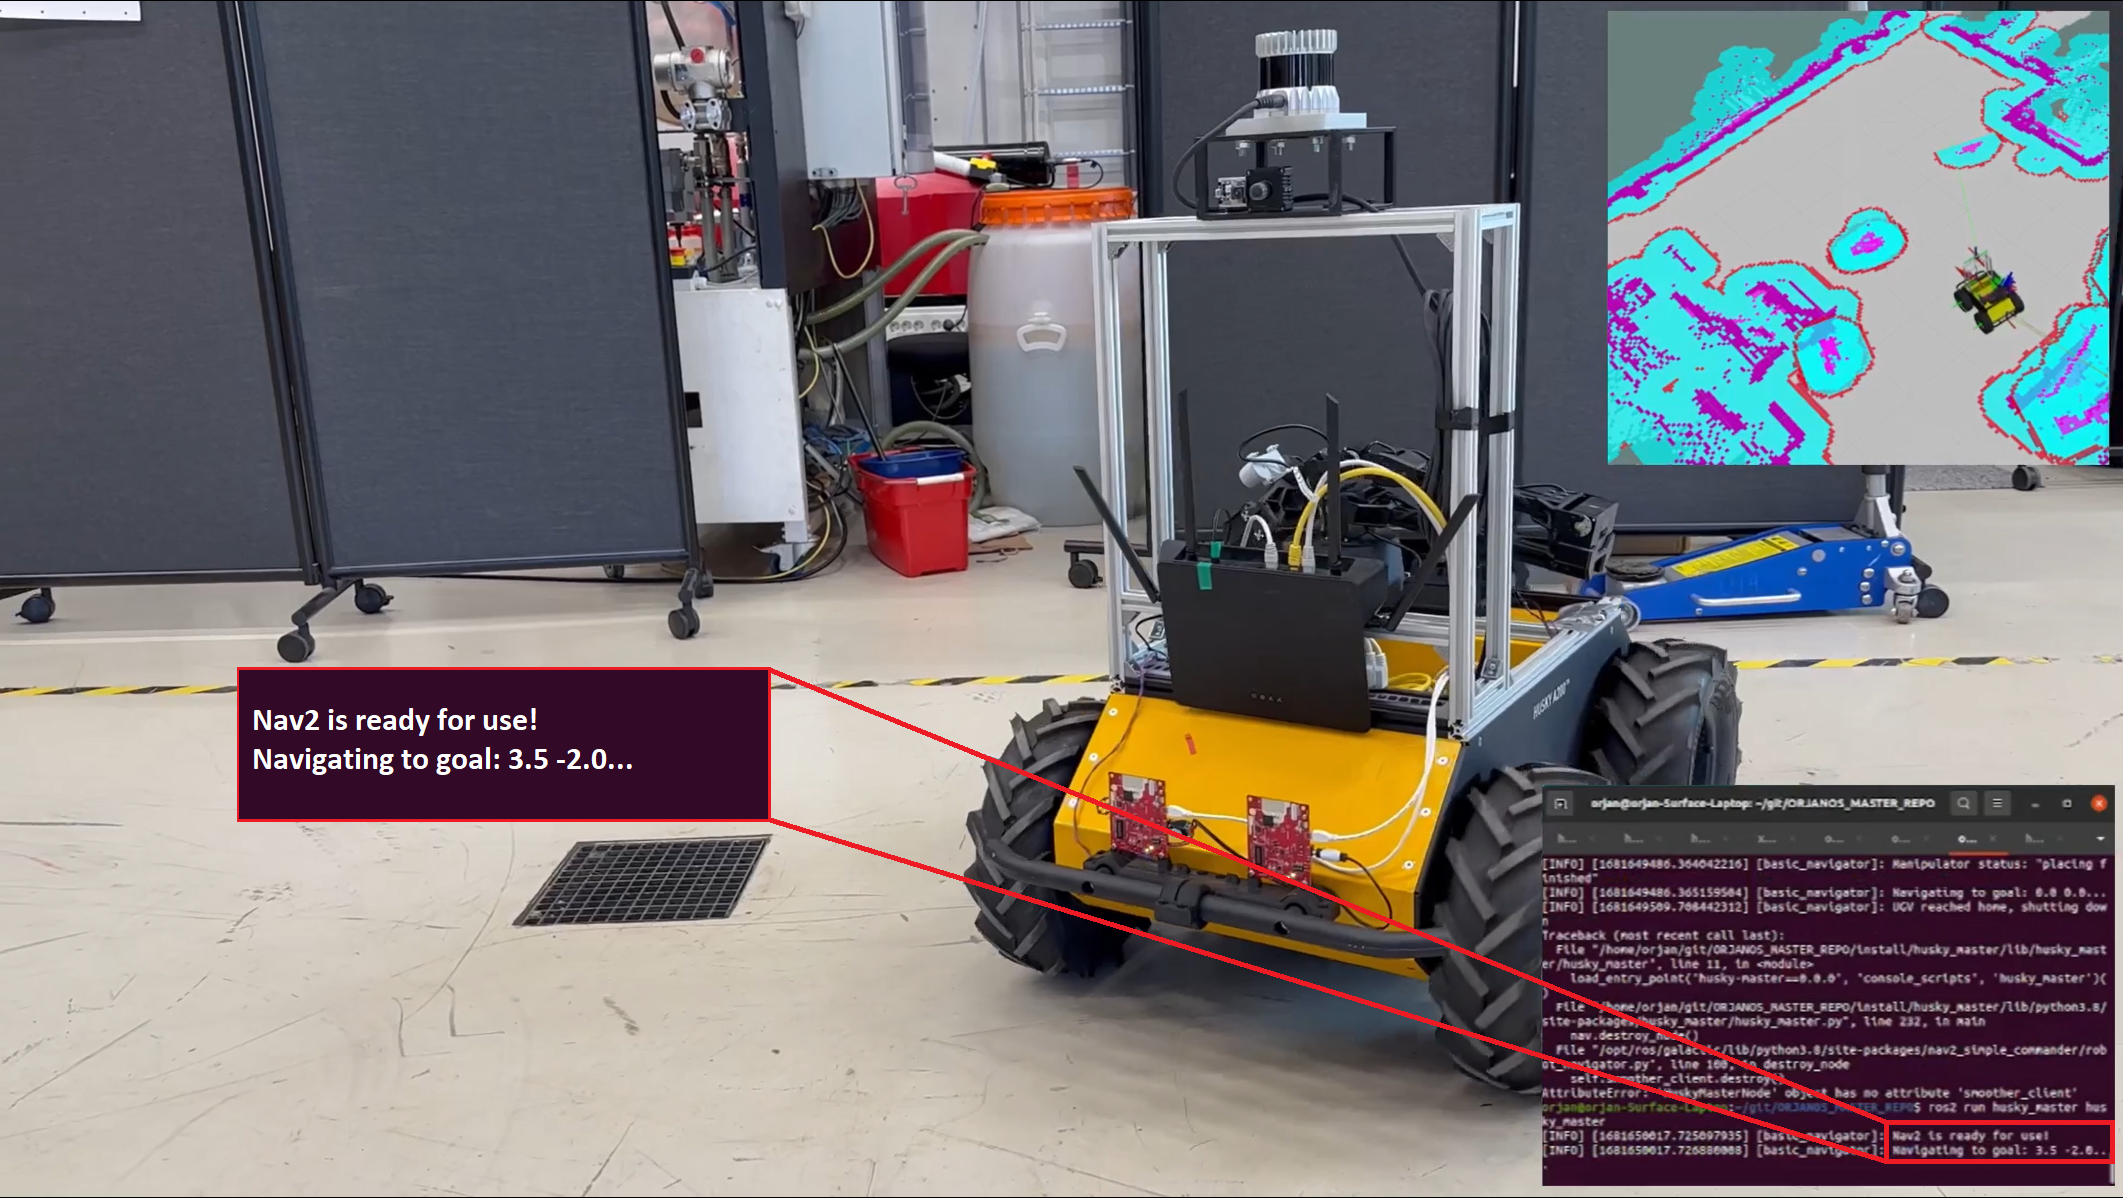
\includegraphics[width = 0.8\textwidth]{Figures/figHuskyFinalExperiment1.png}
  \caption{This figure illustrates initiation of Husky Master Node and navigation towards the first goal during testing. The map in the top right corner corresponds to the actual position of the mobile robot. The terminal window in the lower right corner provides some info about the progress in the warehouse automation pipeline.}
  \label{fig:R:WA:finalExperiment1}
\end{figure}

Figure \ref{fig:R:WA:finalExperiment2} illustrates the picking operation during the warehouse automation task. The mobile robot has reached it's picking pose and is currently performing a picking operation. Interactions between the Husky Master Node and the Pick and Place Node can be seen in the bloated section of the terminal window. The instance figure \ref{fig:R:WA:finalExperiment2} is taken, the manipulator has detected the object, and then placed it's end-effector directly above the object for the computer vision system to get more accurate measurements before picking the object.

\begin{figure}[htp!]
  \centering
  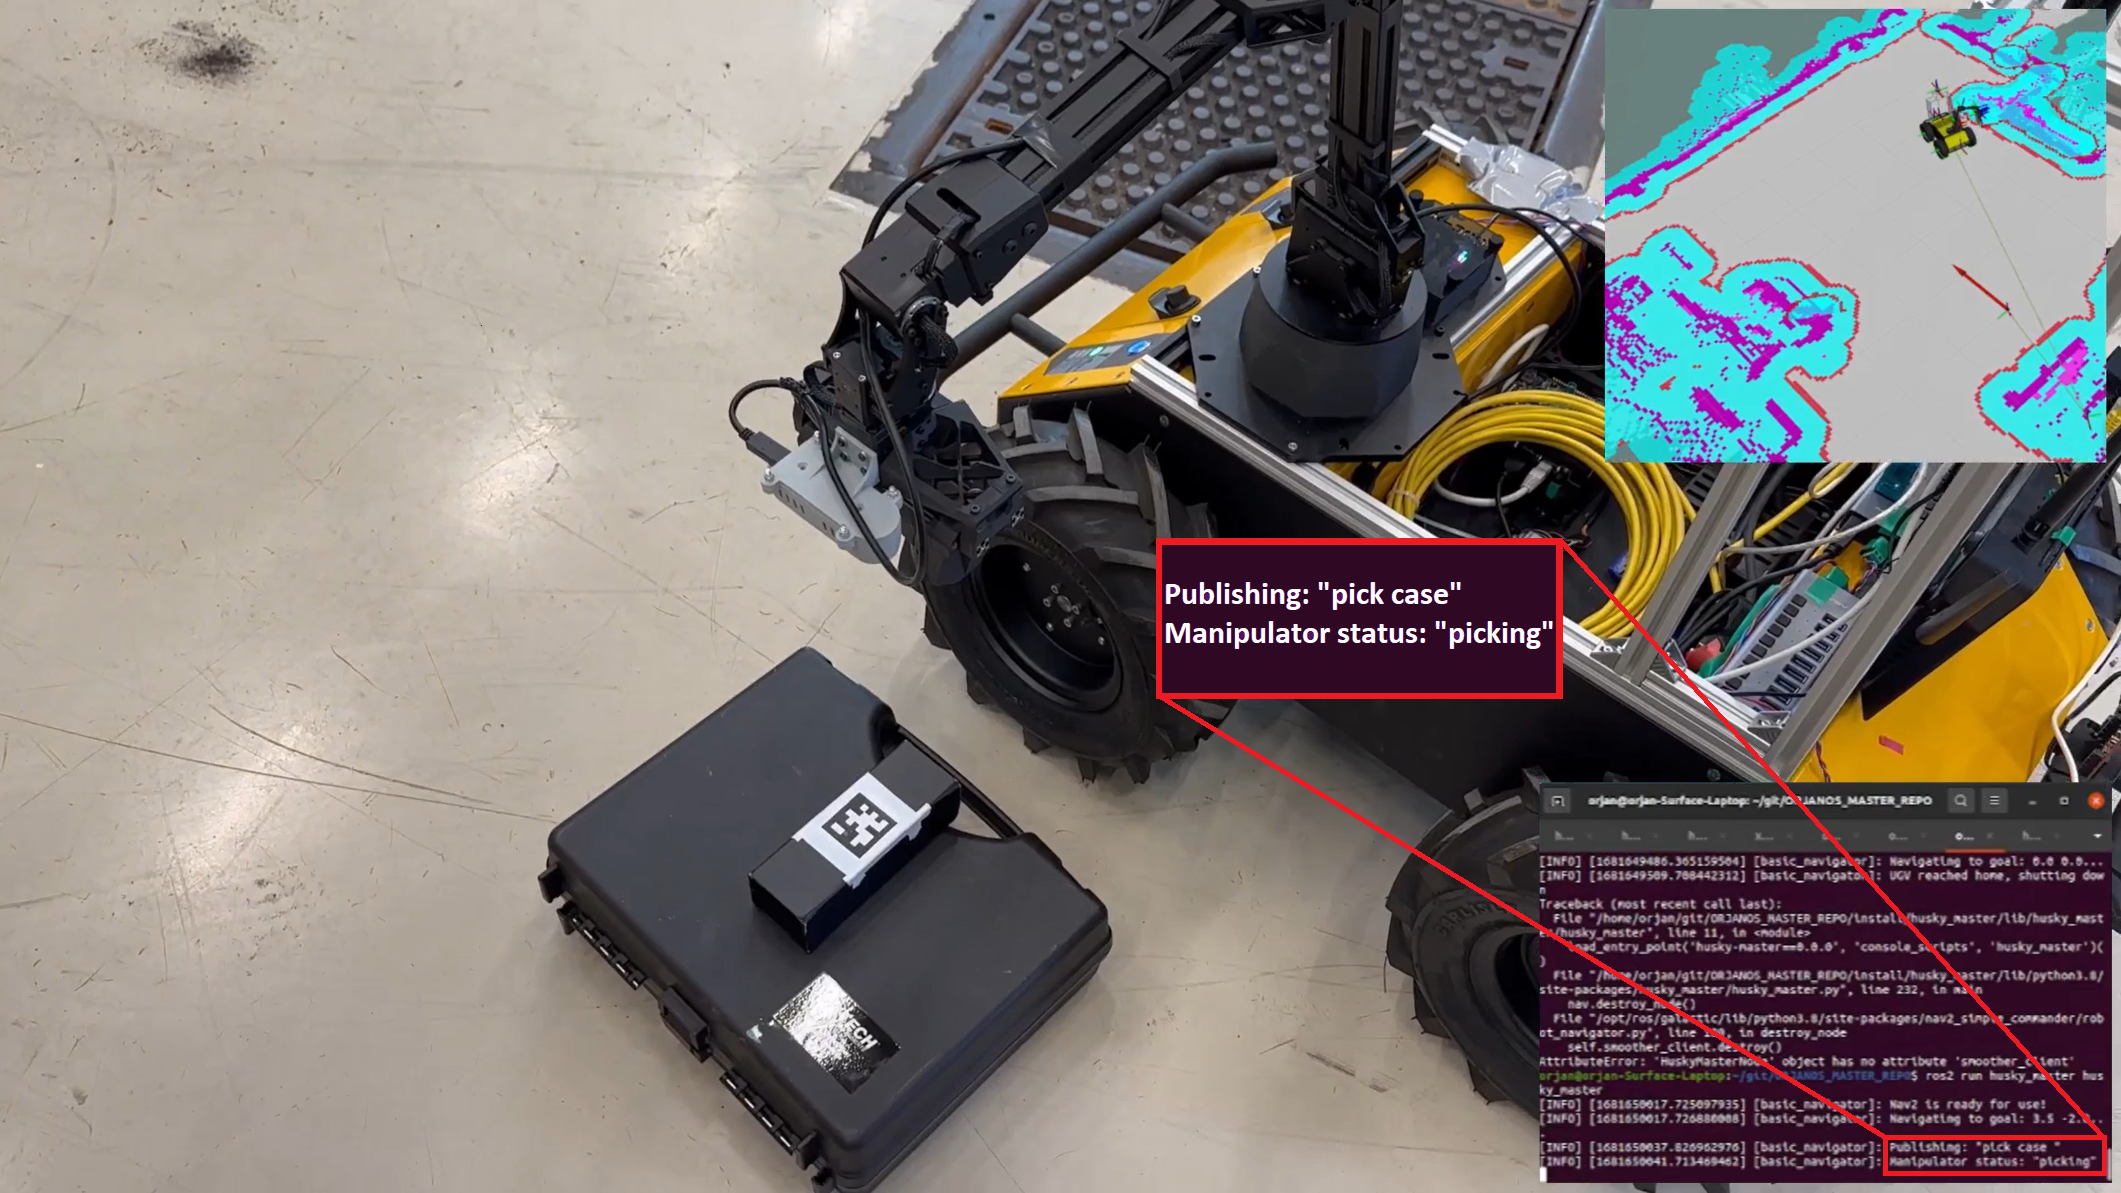
\includegraphics[width = 0.8\textwidth]{Figures/figHuskyFinalExperiment2.png}
  \caption{This figure illustrates picking operation during the warehouse automation task. In this instance, the manipulator has positioned itself directly above the object to give a more accurate measurement before picking. Relevant command and feedback between the Husky Master node and Pick and Place node can be seen in the bloated section from the terminal.}
  \label{fig:R:WA:finalExperiment2}
\end{figure}

% \begin{figure}[htp!]
%   \centering
%   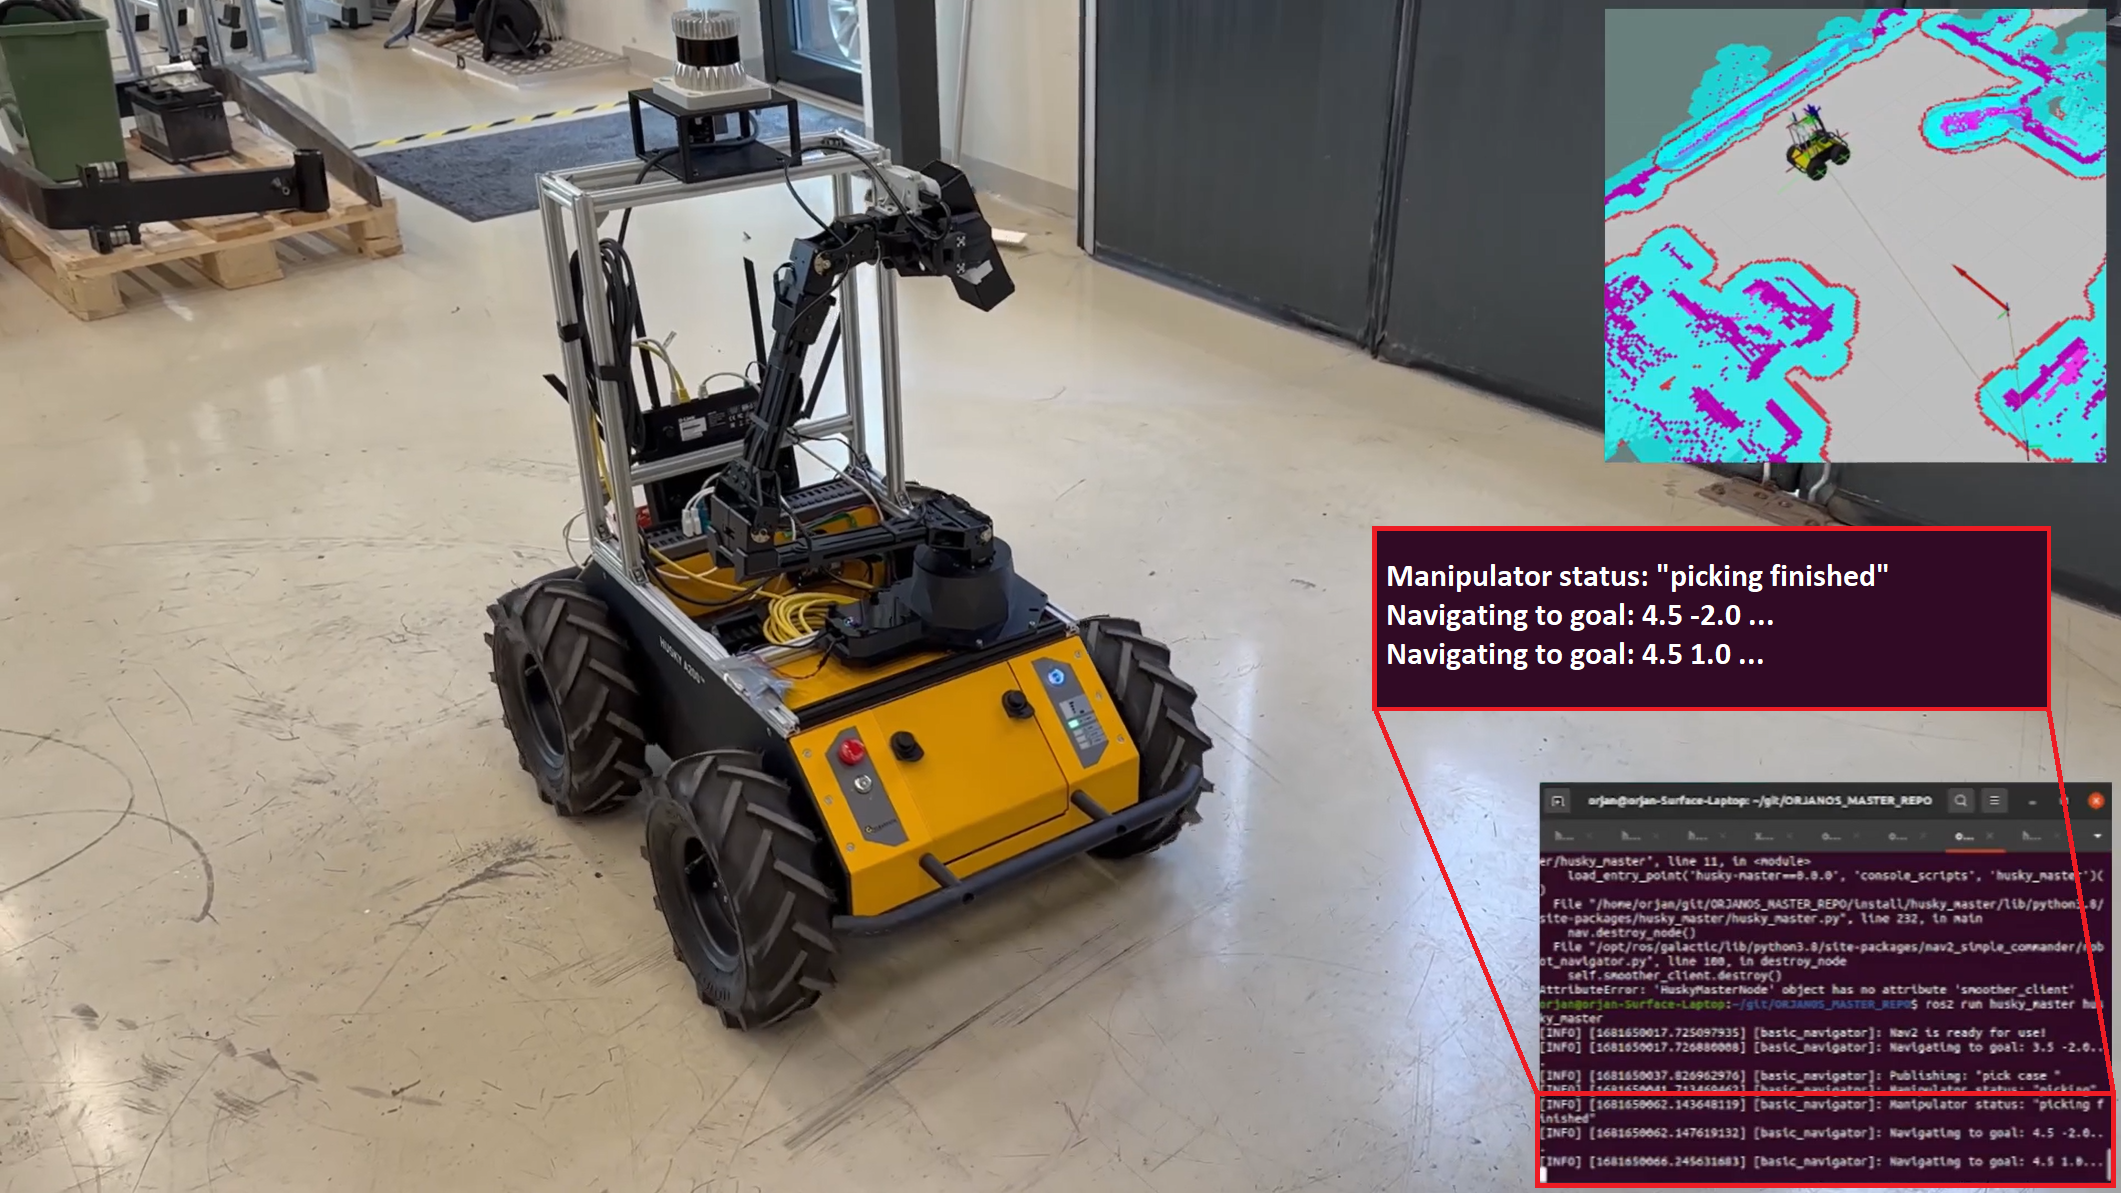
\includegraphics[width = 0.8\textwidth]{Figures/figHuskyFinalExperiment3.png}
%   \caption{This figure illustrates }
%   \label{fig:R:WA:finalExperiment3}
% \end{figure}

The placing operation of the warehouse automation task is shown in figure \ref{fig:R:WA:finalExperiment4}. As with figure \ref{fig:R:WA:finalExperiment2}, interactions between the Husky Master Node and the Pick and Place Node can be seen in the bloated terminal section. The object has been dropped to the floor moments before figure \ref{fig:R:WA:finalExperiment4} is captured.

\begin{figure}[htp!]
  \centering
  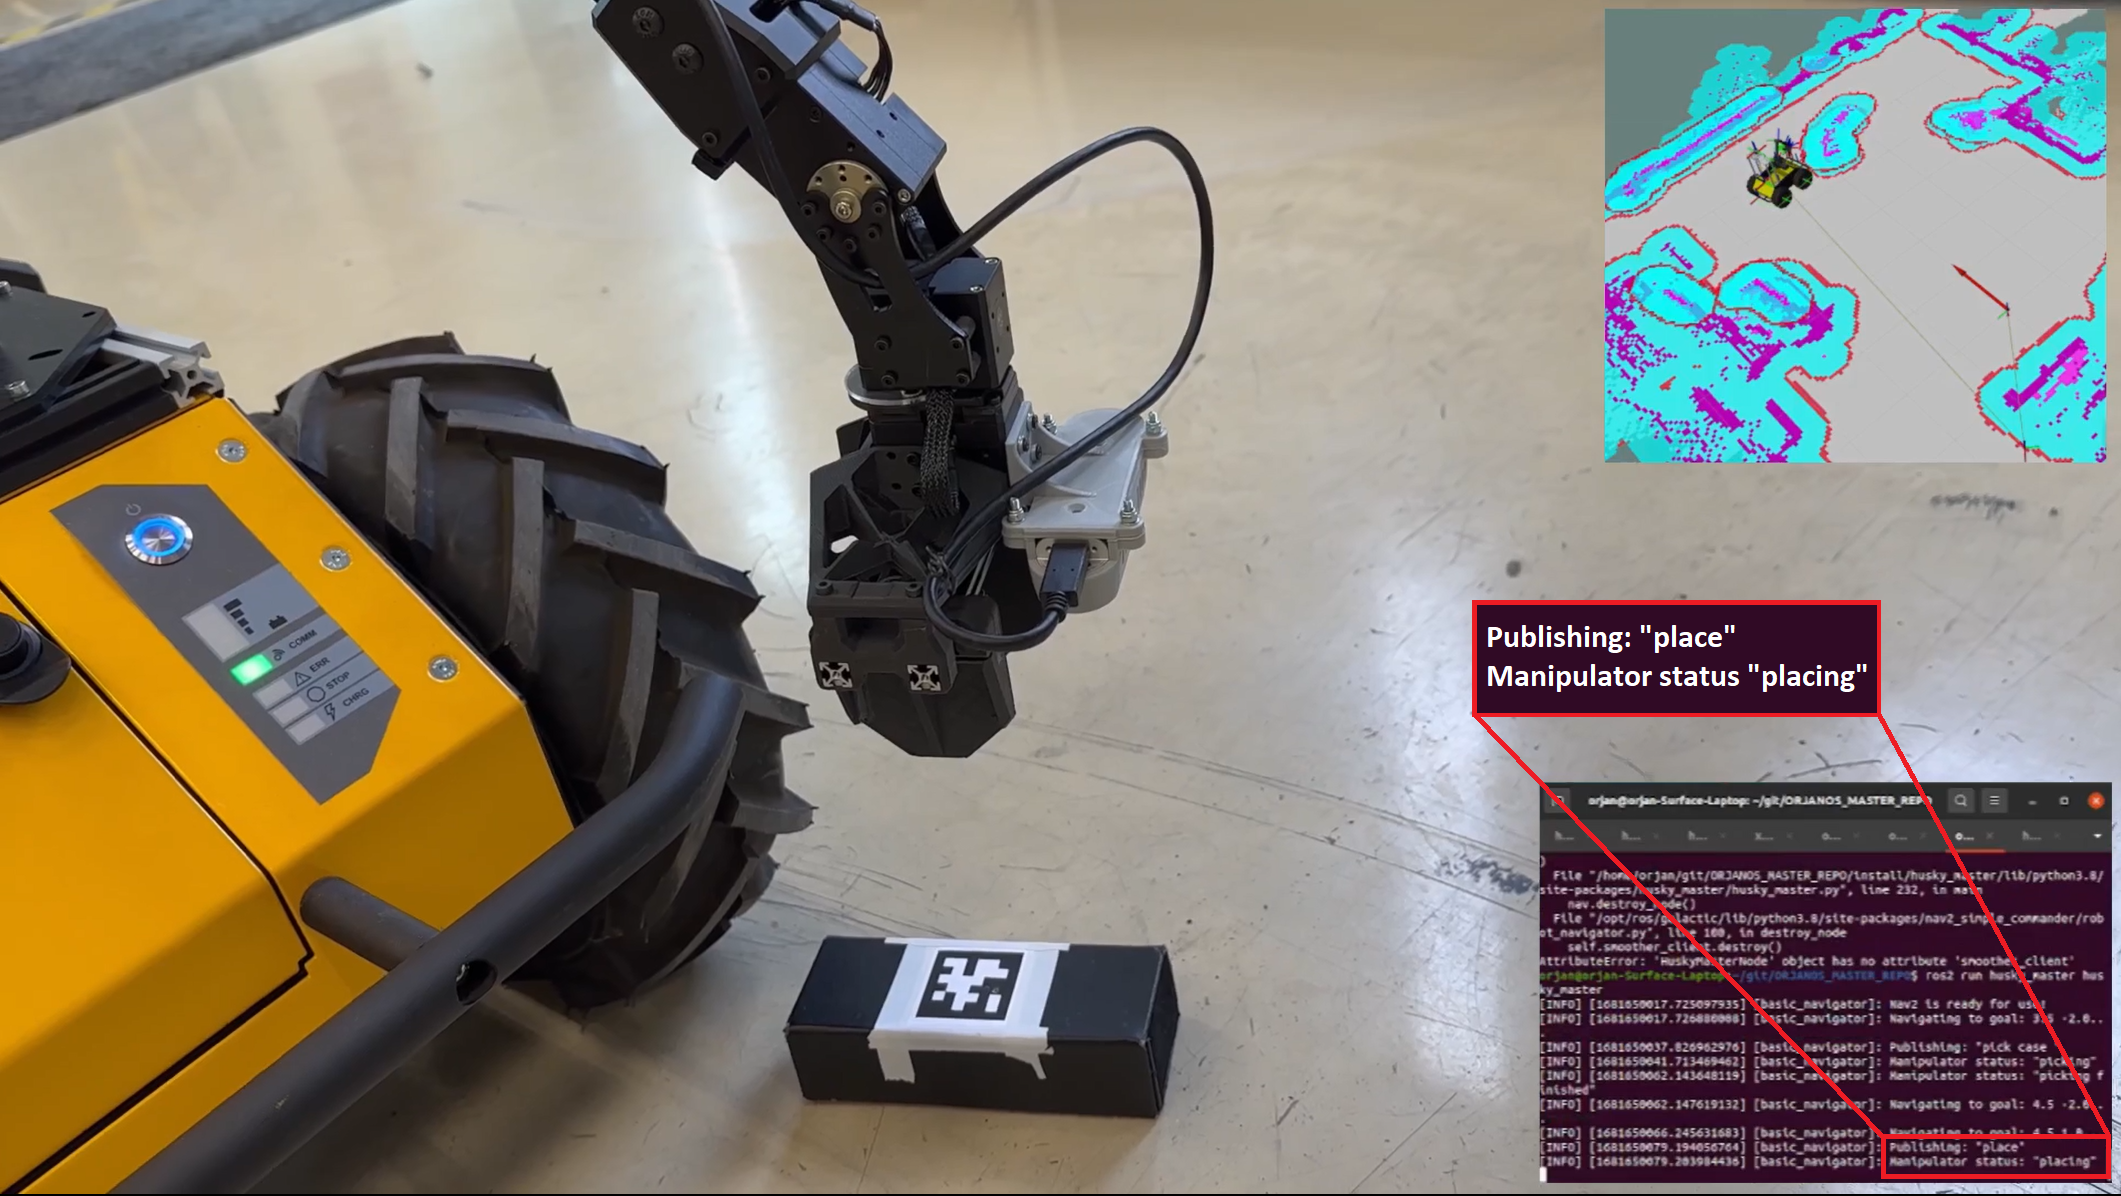
\includegraphics[width = 0.8\textwidth]{Figures/figHuskyFinalExperiment4.png}
  \caption{This figure illustrates the placing operation during the warehouse automation task. Notice from the map in the top left corner that the mobile robot has moved to a different location. Relevant command and feedback between the Husky Master node and Pick and Place node can be seen in the bloated terminal.}
  \label{fig:R:WA:finalExperiment4}
\end{figure}

After placing is finished, the mobile should return to it's starting position. This is illustrated in figure \ref{fig:R:WA:finalExperiment5}. There is a red arrow pointing at a coordinate frame in figure \ref{fig:R:WA:finalExperiment5}. This is the last known coordinate of the placed object. The bloated terminal section indicates that the placing operation is finished, and that the robot is moving to "0.0 0.0 ...", in other words, start position.

\begin{figure}[htp!]
  \centering
  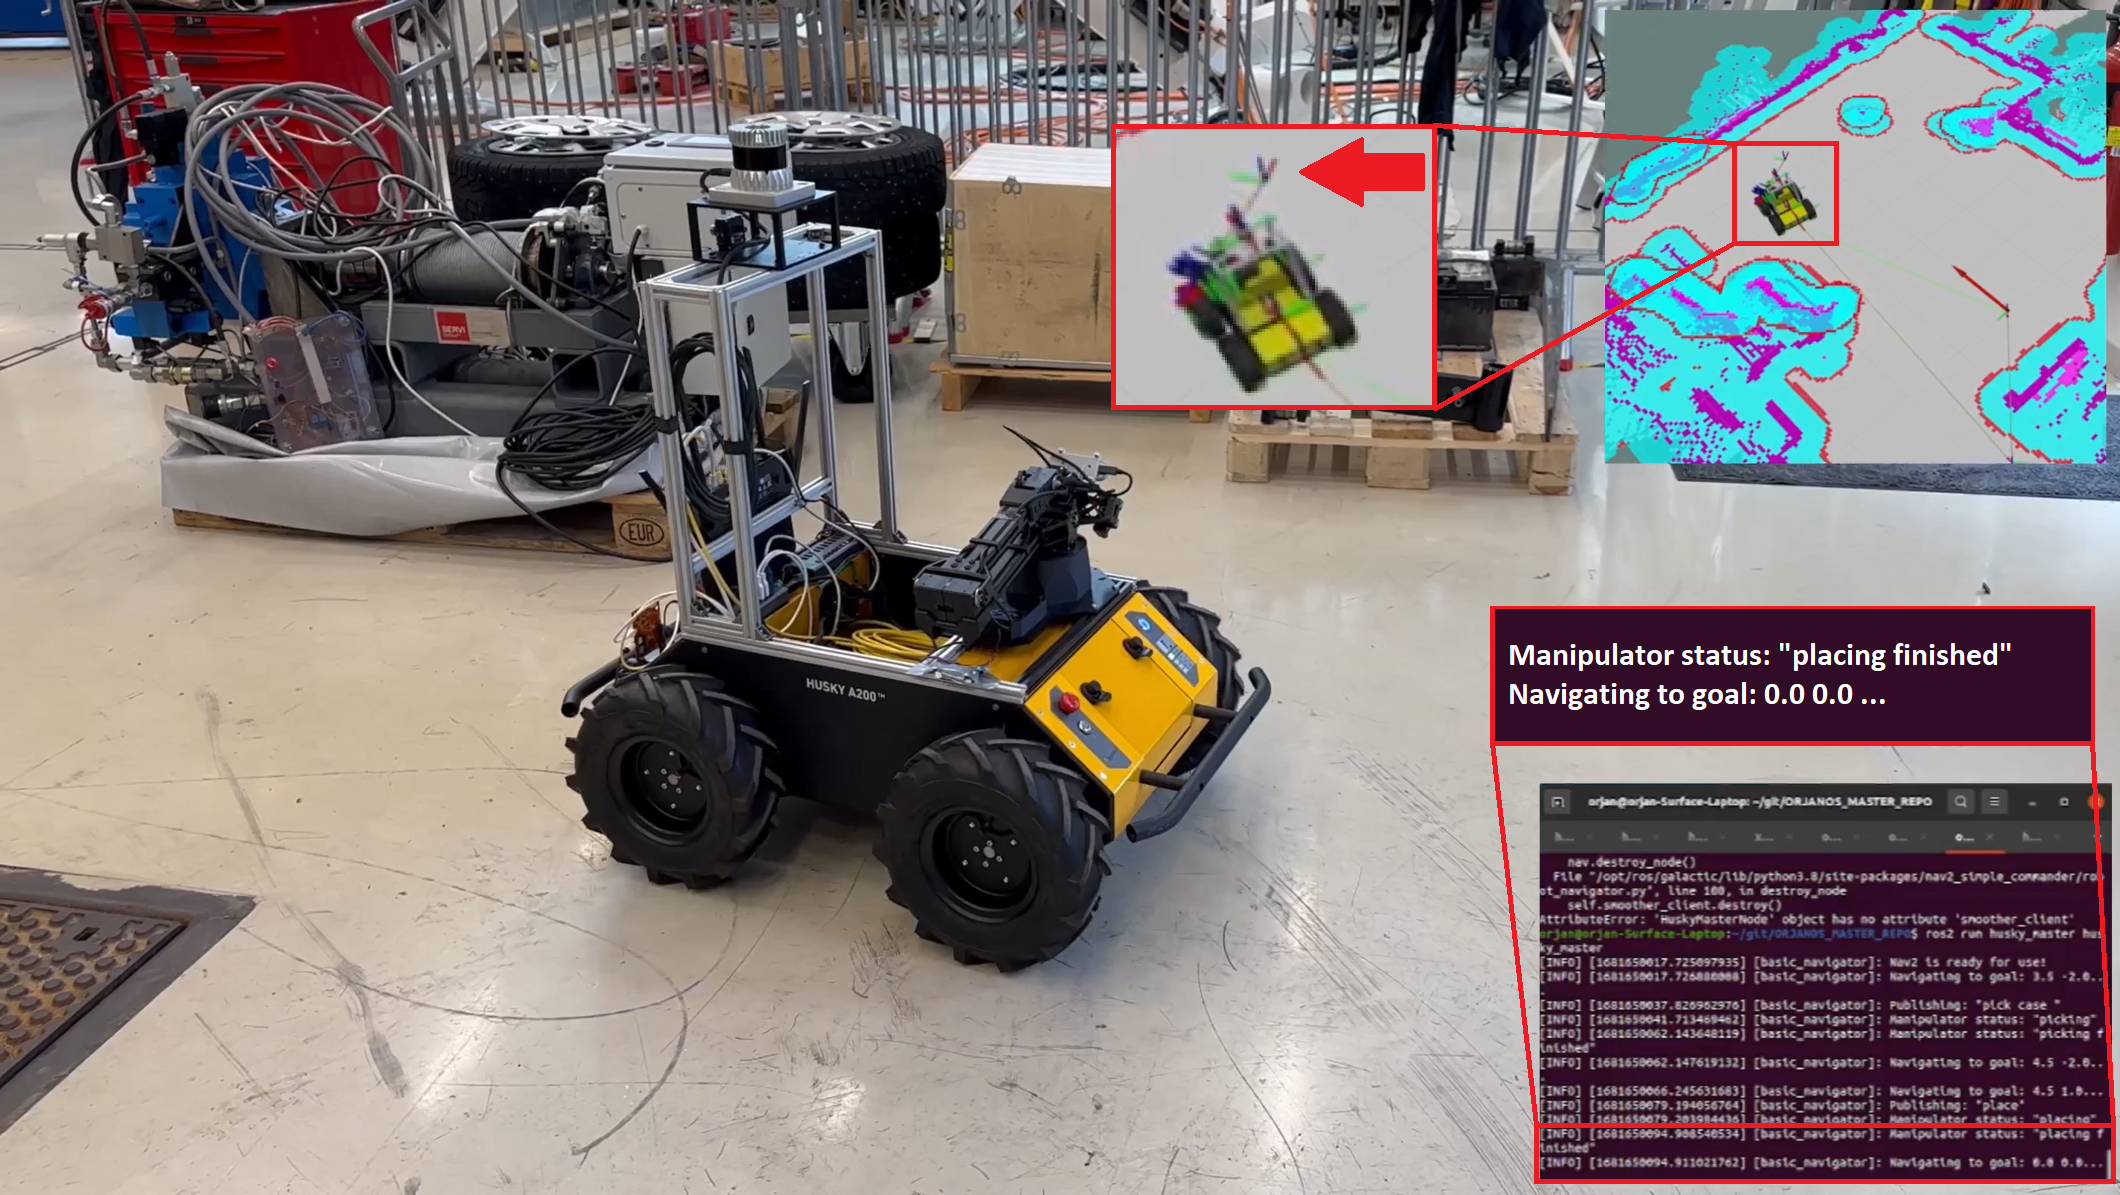
\includegraphics[width = 0.8\textwidth]{Figures/figHuskyFinalExperiment5.png}
  \caption{This figure illustrates that the mobile robot is navigating back to it's starting pose after placing the object. The bloated section from the map has a red arrow pointing at a coordinate frame behind the mobile robot. This is the last known coordinate of the placed object.}
  \label{fig:R:WA:finalExperiment5}
\end{figure}

\FloatBarrier
\subsection{Simulation Experiment}
Top-level system testing has been performed in a Gazebo simulation of the robotic system as well. This has been done by first bringing up the mobile robot simulation and the pick and place simulation. Then, a simple Gazebo environment is set up with some simple shapes, before SLAM and navigation is launched with the parameters provided in the custom ROS 2 package \lstinline{husky_group}. Finally, the top-level system is launched by running the Husky Master Node. As the computer vision system is not simulated, the detected object is represented by a static transformation from the manipulator base. Figure \ref{fig:R:WA:simTopLevel0}, \ref{fig:R:WA:simTopLevel1}, \ref{fig:R:WA:simTopLevel2} and \ref{fig:R:WA:simTopLevel3} illustrates the results of these tests. In all the four figures, the gazebo environment is illustrated in the lower right corner and a digital twin of the complete system is visualised in the top right corner. The terminal in the lower left corner gives information about progress and current status on the warehouse automation scenario.

Figure \ref{fig:R:WA:simTopLevel0} illustrates initiation of the warehouse scenario simulation experiment. The terminal in the lower right corner indicates that the husky master node is being initiated. It can also be seen that the manipulator is in it's sleep position.

\begin{figure}[htp!]
  \centering
  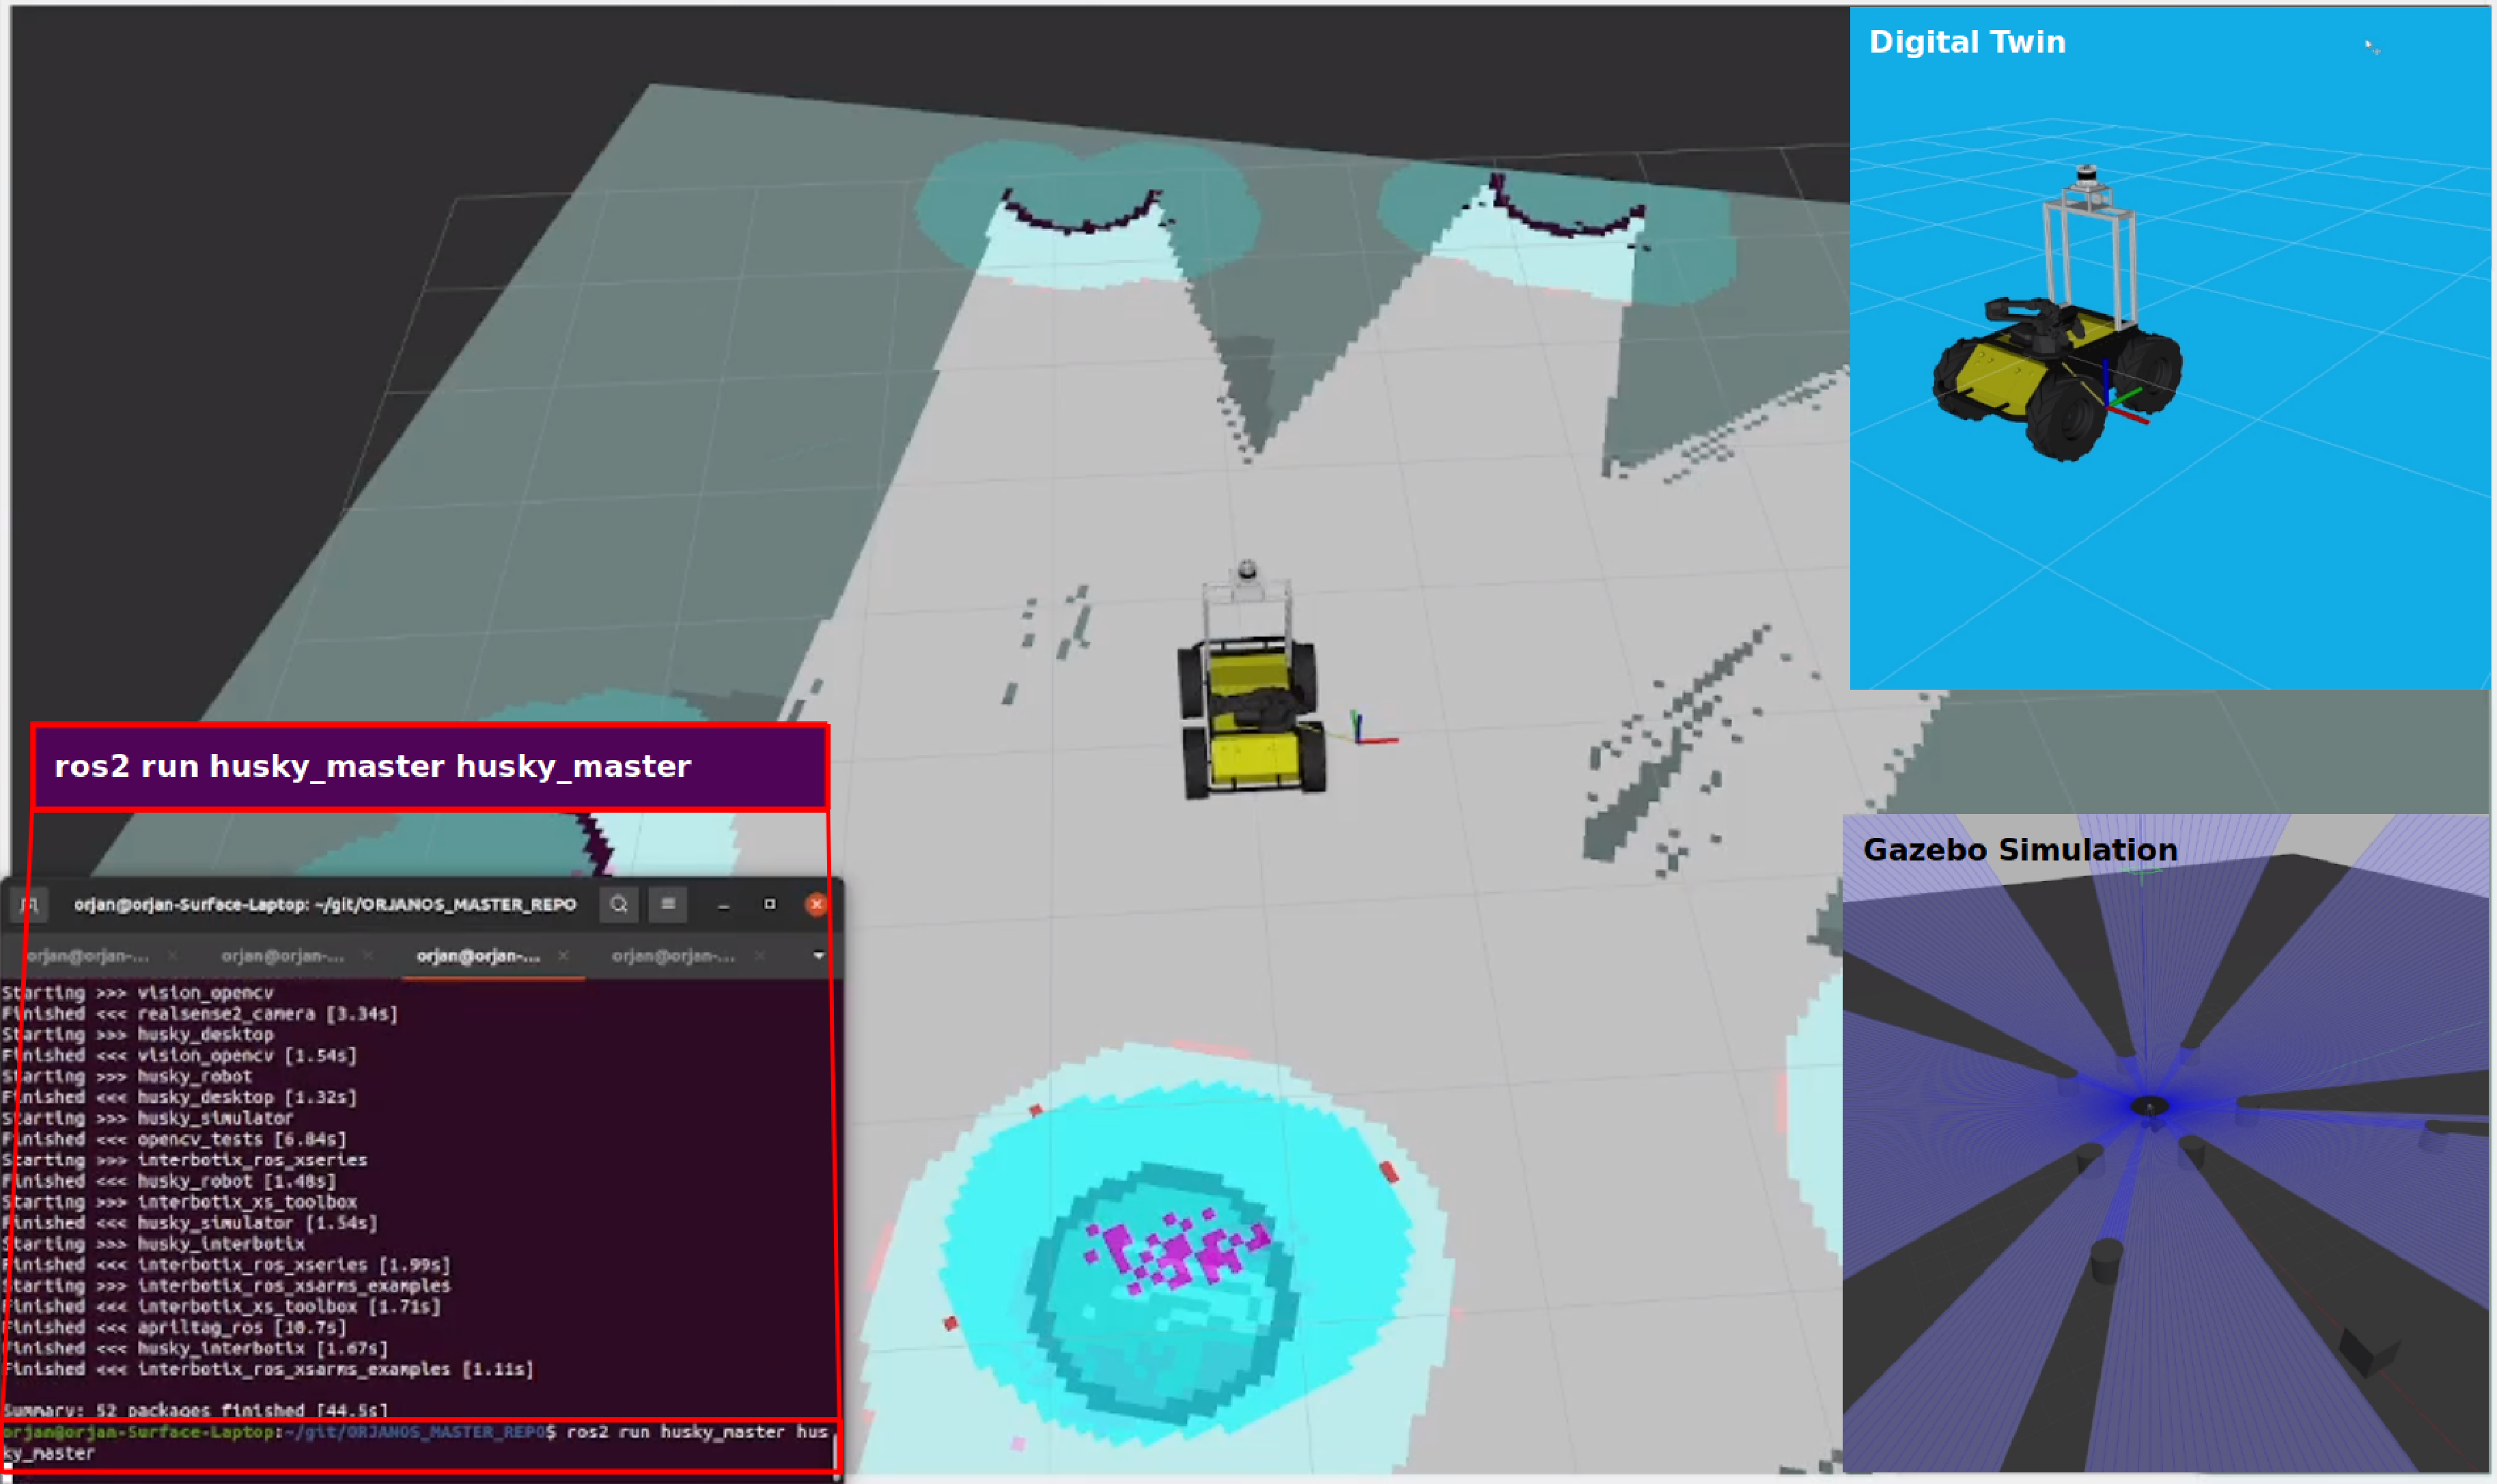
\includegraphics[width = 0.85\textwidth]{Figures/figSimTopLevel0.pdf}
  \caption{This figure illustrates initiation of top warehouse automation scenario testing in a simulation environment. \textbf{Top right:} digital twin of complete robotic system. \textbf{Lower right:} visualisation of gazebo simulation environment. \textbf{Lower left:} terminal window including bloated view of important information.}
  \label{fig:R:WA:simTopLevel0}
\end{figure}

Figure \ref{fig:R:WA:simTopLevel1} illustrates picking operation during the warehouse scenario simulation experiment. It can be seen from both the map and the Gazebo window that the mobile robot has relocated itself. The terminal window indicates that the picking operation is under way.

\begin{figure}[htp!]
  \centering
  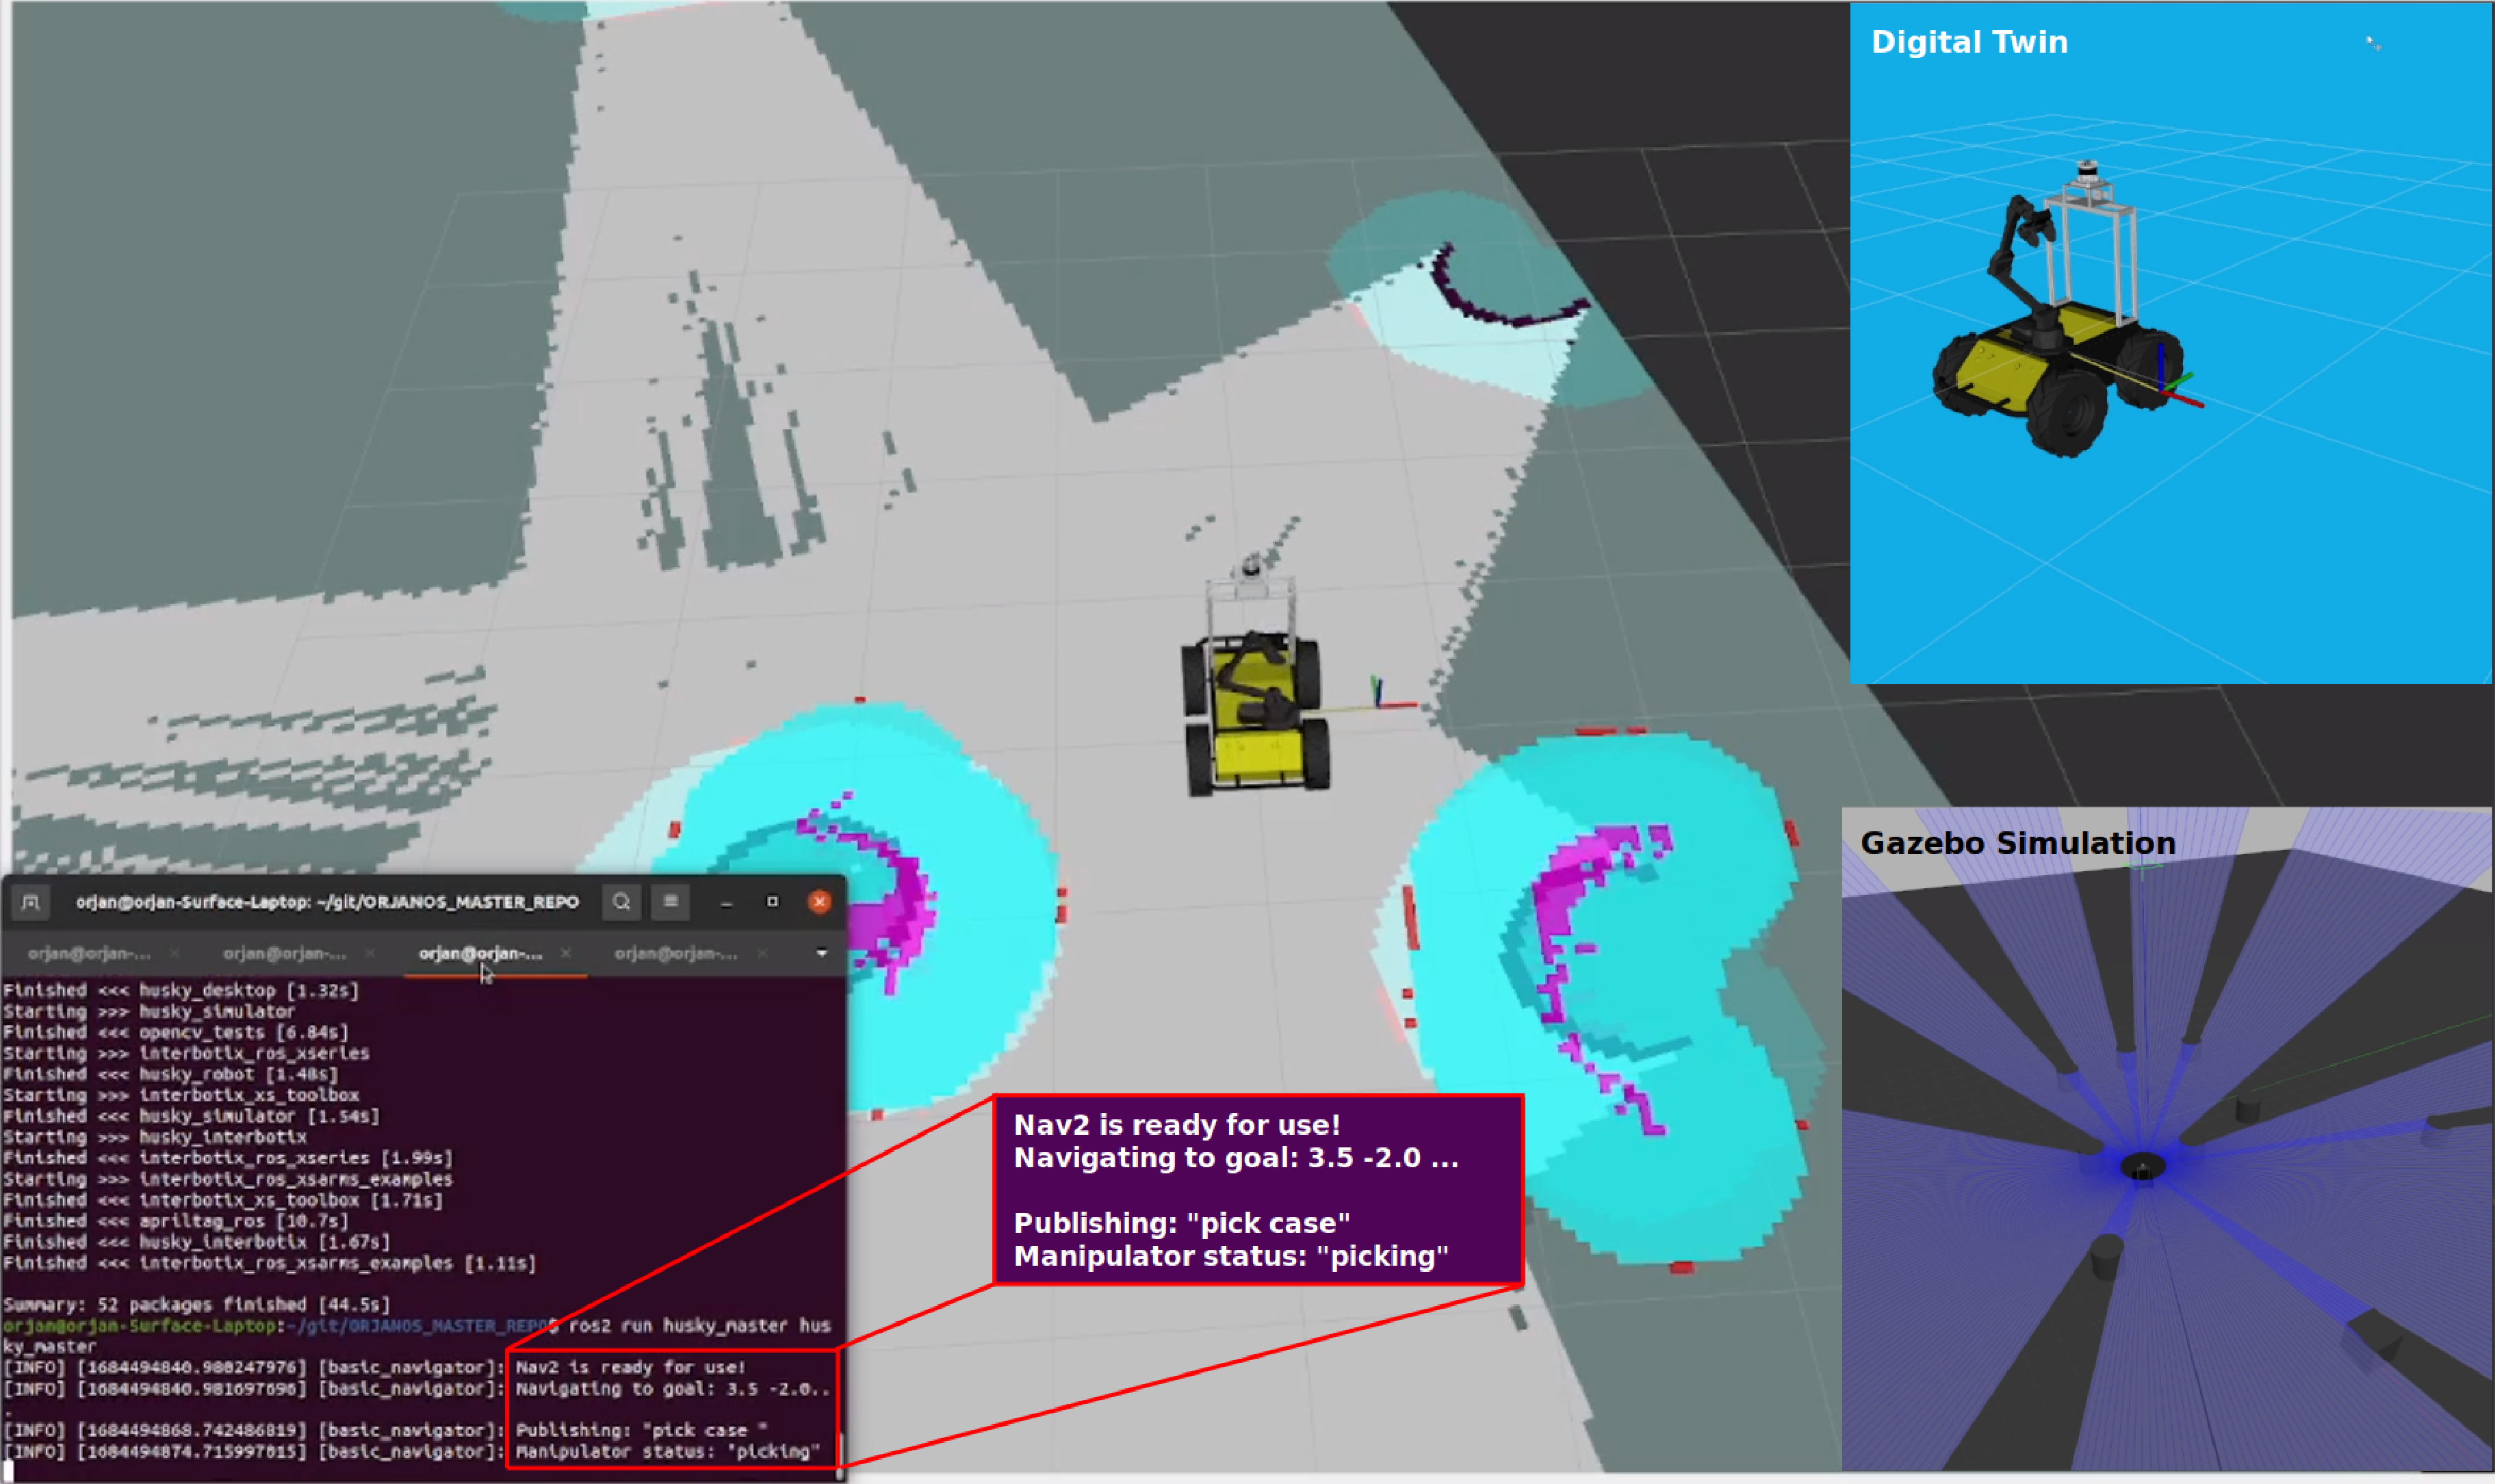
\includegraphics[width = 0.85\textwidth]{Figures/figSimTopLevel1.pdf}
  \caption{This figure illustrates picking operation during testing of top-level system on simulation of the robot in a Gazebo environment. \textbf{Top right:} digital twin of complete robotic system. \textbf{Lower right:} visualisation of gazebo simulation environment. \textbf{Lower left:} terminal window including bloated view of important information.}
  \label{fig:R:WA:simTopLevel1}
\end{figure}

Placing operation is illustrated in figure \ref{fig:R:WA:simTopLevel2}. Again, it can be seen from the map and the Gazebo window that the robot has relocated itself. The terminal confirms that the placing operation is being performed.

\begin{figure}[htp!]
  \centering
  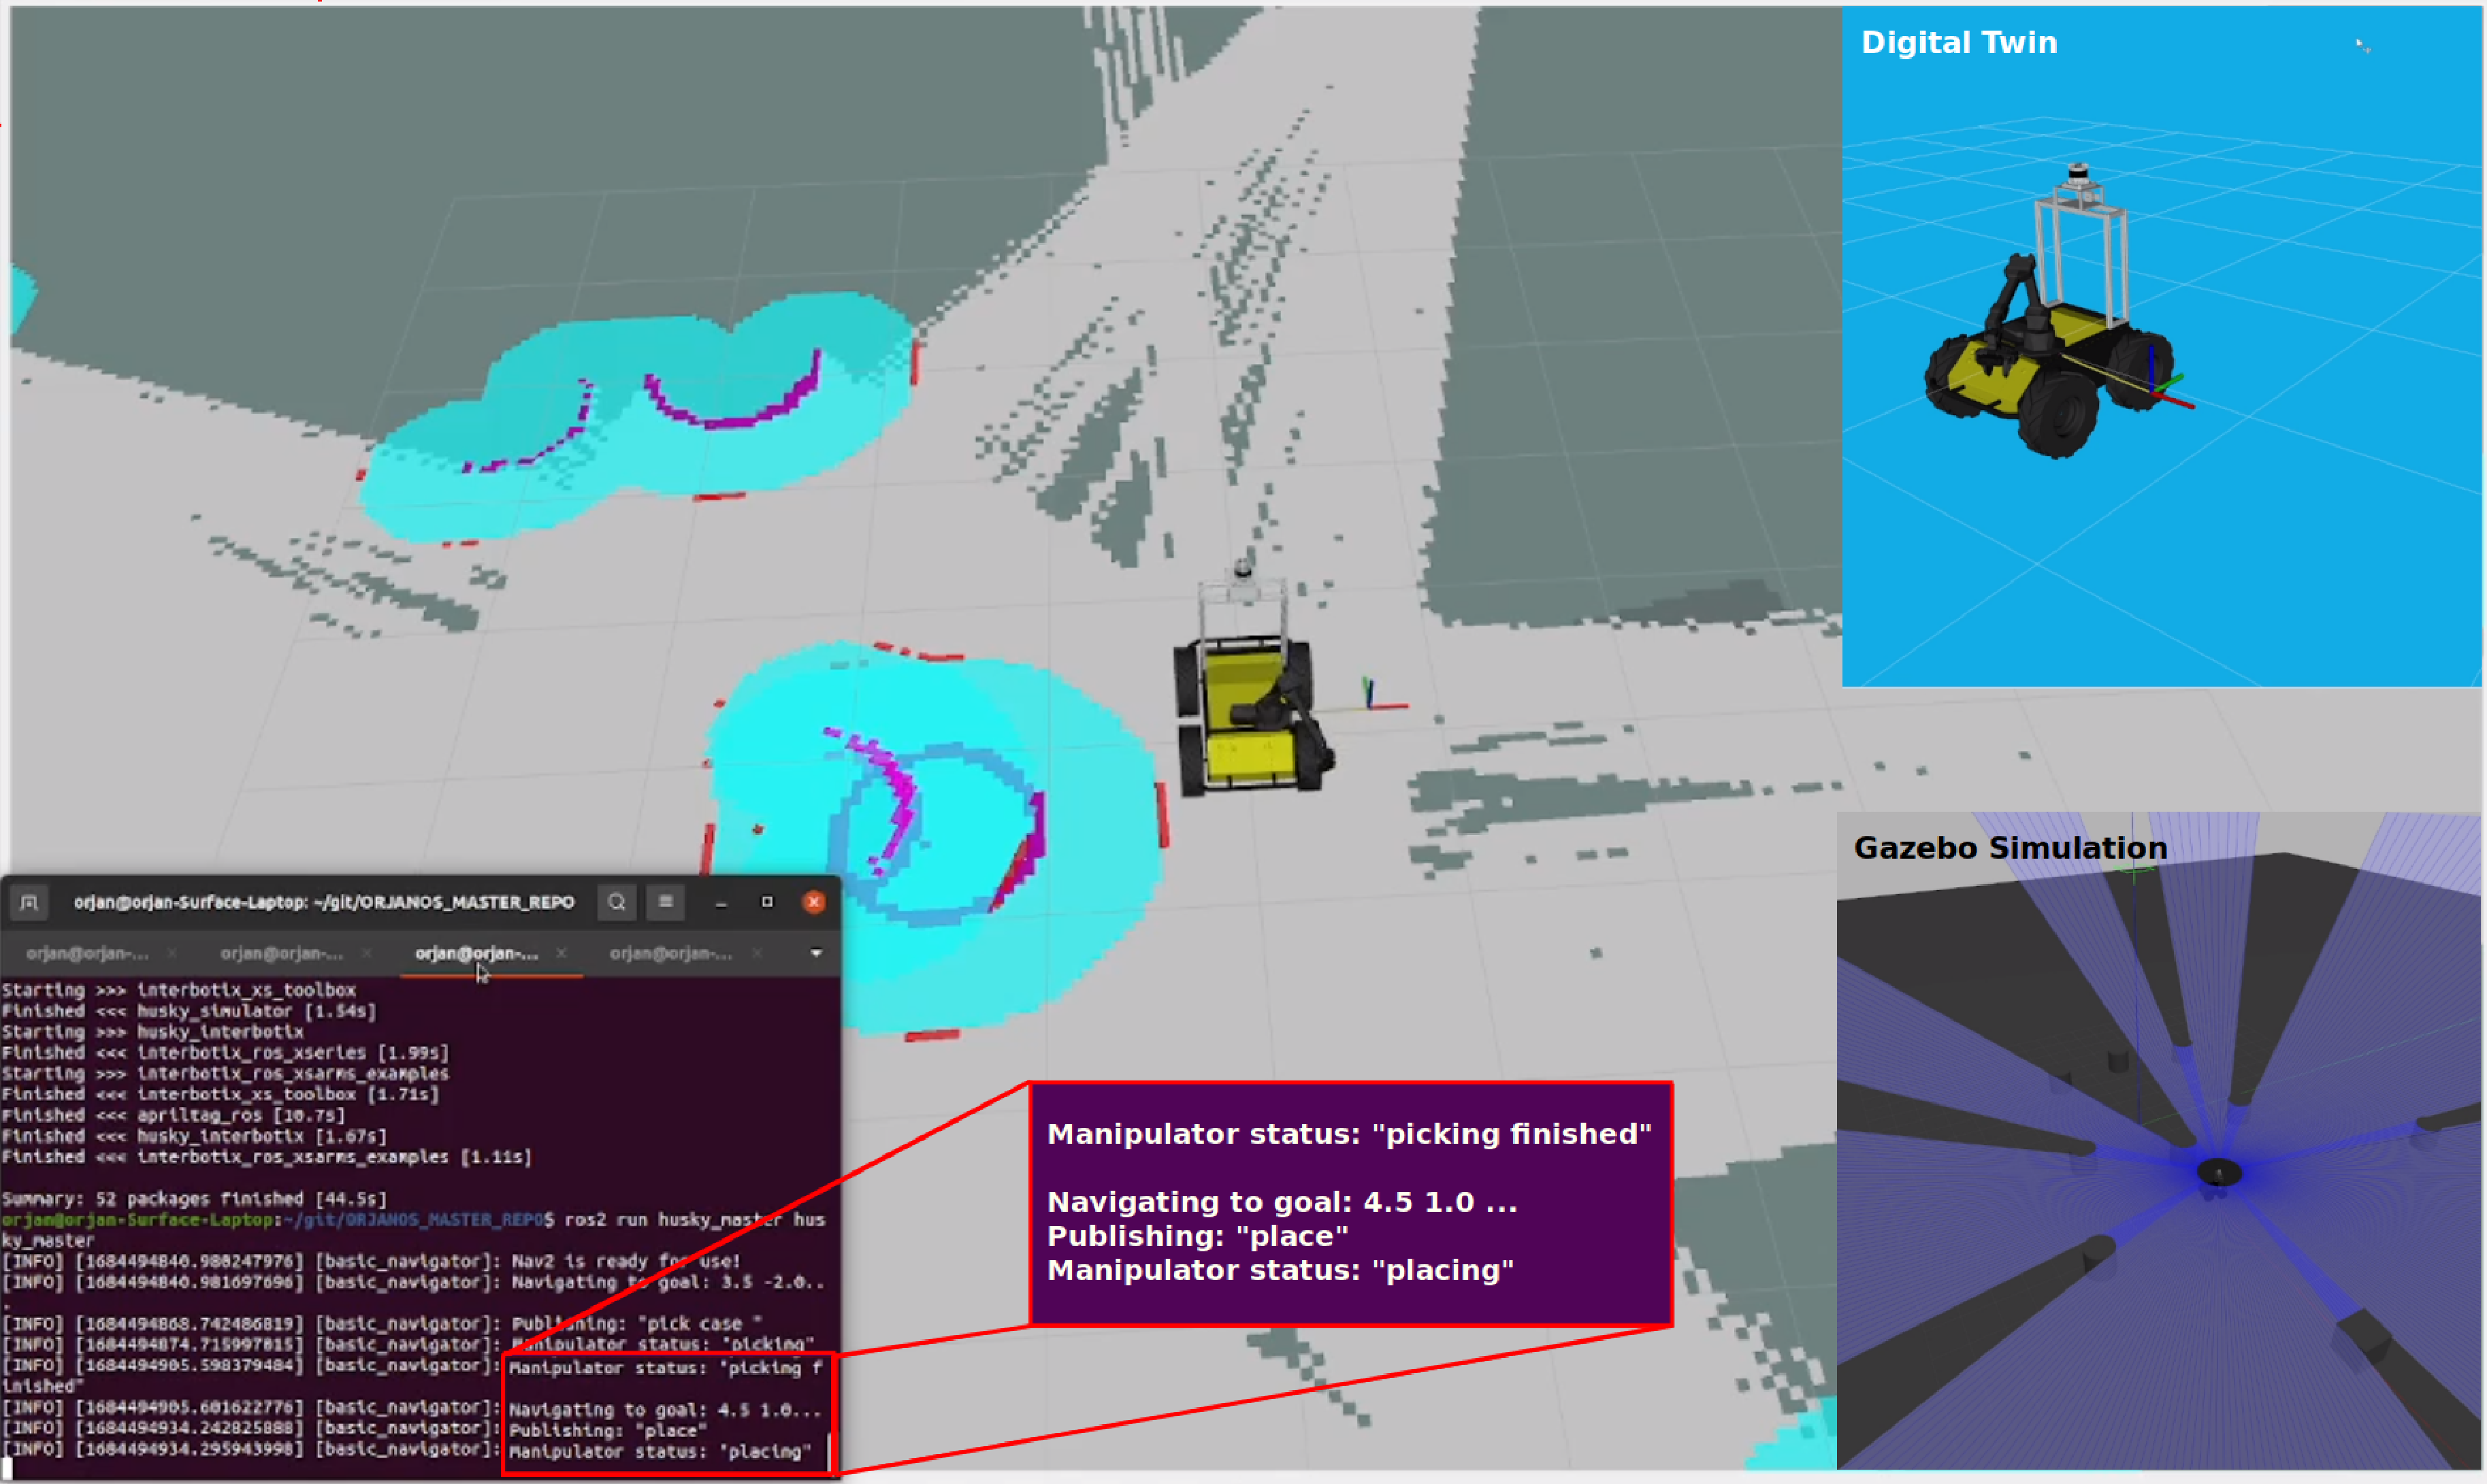
\includegraphics[width = 0.85\textwidth]{Figures/figSimTopLevel2.pdf}
  \caption{This figure illustrates placing operation during testing of top-level system on simulation of the robot in a Gazebo environment. \textbf{Top right:} digital twin of complete robotic system. \textbf{Lower right:} visualisation of gazebo simulation environment. \textbf{Lower left:} terminal window including bloated view of important information.}
  \label{fig:R:WA:simTopLevel2}
\end{figure}

Figure \ref{fig:R:WA:simTopLevel3} shows the robotic system at it's final pose. It can be seen in the gazebo window that the final pose is not the same as the start pose shown in figure \ref{fig:R:WA:simTopLevel0}. Looking at the terminal, the node reports that the UGV has reached home and is shutting down.

\begin{figure}[htp!]
  \centering
  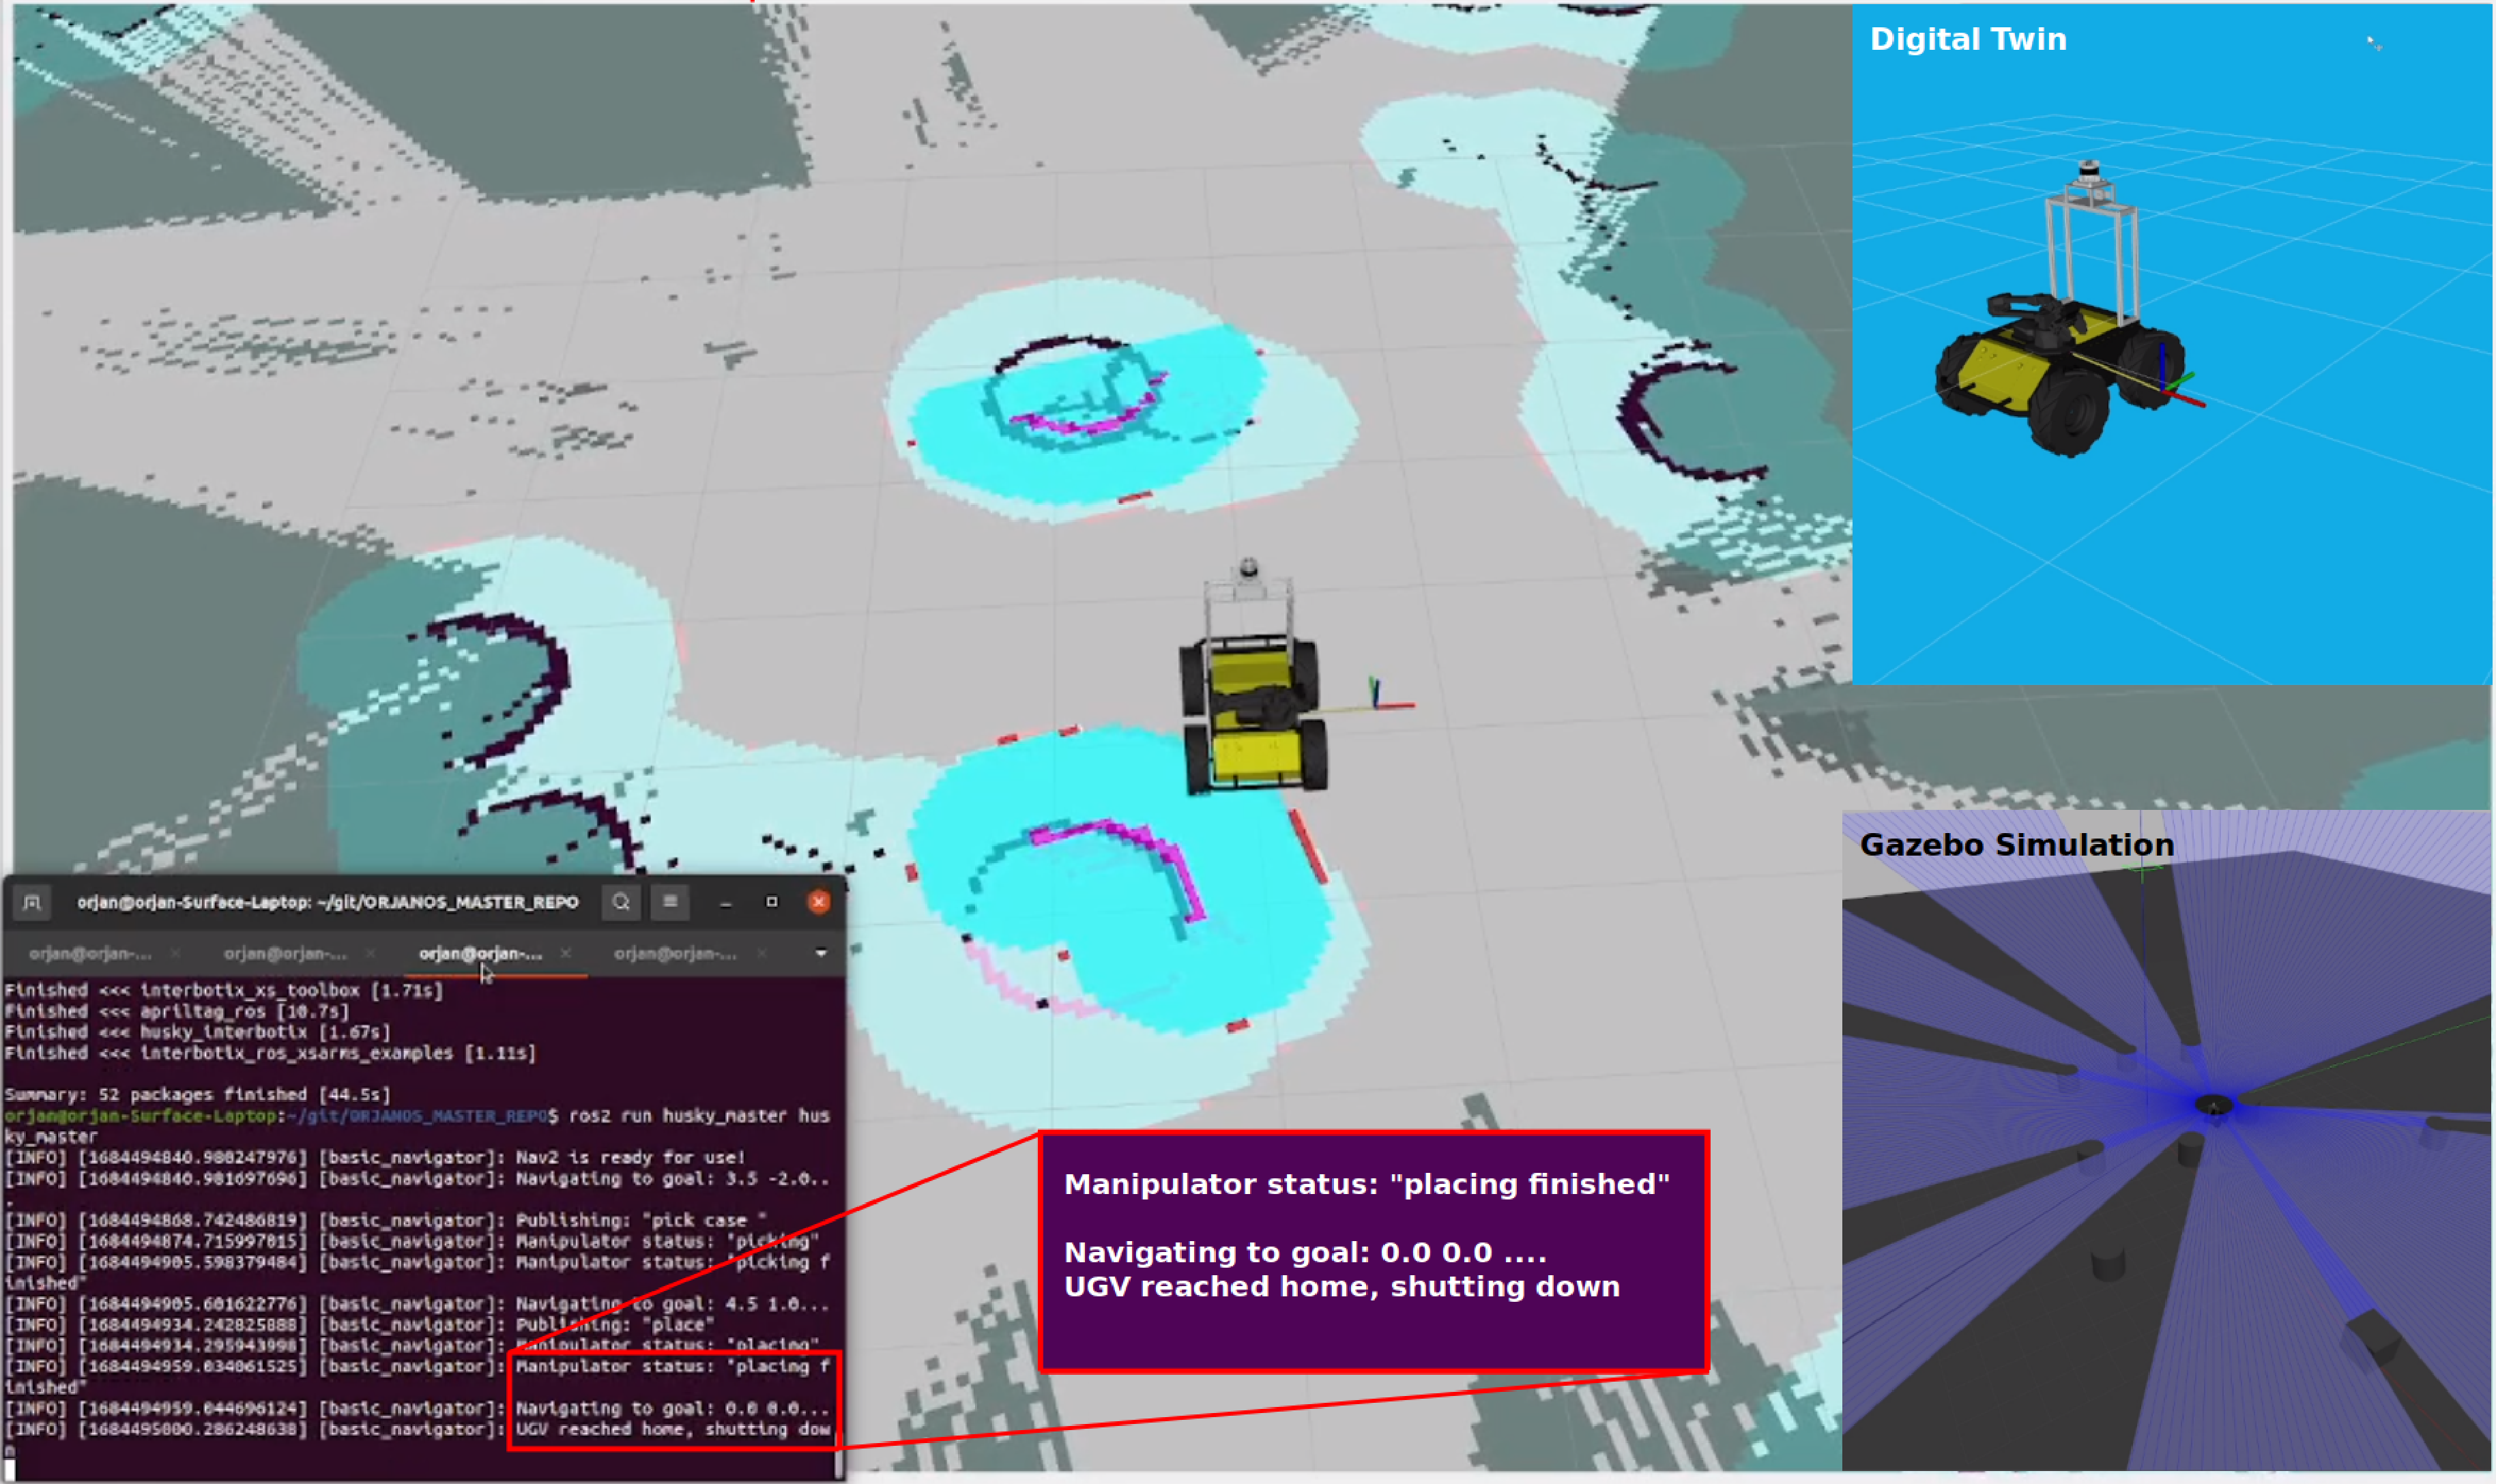
\includegraphics[width = 0.85\textwidth]{Figures/figSimTopLevel3.pdf}
  \caption{This figure illustrates testing of top-level system on simulation of the robot in a Gazebo environment. In this instance, the robot has reported that it has reached home and is shutting down. \textbf{Top right:} digital twin of complete robotic system. \textbf{Lower right:} visualisation of gazebo simulation environment. \textbf{Lower left:} terminal window including bloated view of important information.}
  \label{fig:R:WA:simTopLevel3}
\end{figure}

\FloatBarrier
\subsection{TurtleBot3 Simulation Experiment}
To test the flexibility of the top-level system for other mobile robotic platforms, the top-level system was tested together with a TurtleBot3 (popular differential drive robot for ROS and ROS 2) simulation and a virtual VX300 manipulator arm. The test is performed by launching a standard TurtleBot3 navigation simulation provided by NAV2, before launching a virtual Interbotix VX300 manipulator. The Husky Master Node is then launched to orchestrate the sequence. As there are no vision system, the detected object pose is simulated with a static transformation from the manipulators base. Figure \ref{fig:R:WA:simTBTopLevel2} provides an illustration of this test, where it can be seen that similar messages as the ones from the physical test is being displayed in the terminal window. A video of this experiment can be seen in 2x speed \href{https://youtu.be/_Dy3rSTHWYo}{here}. 

\begin{figure}[htp!]
  \centering
  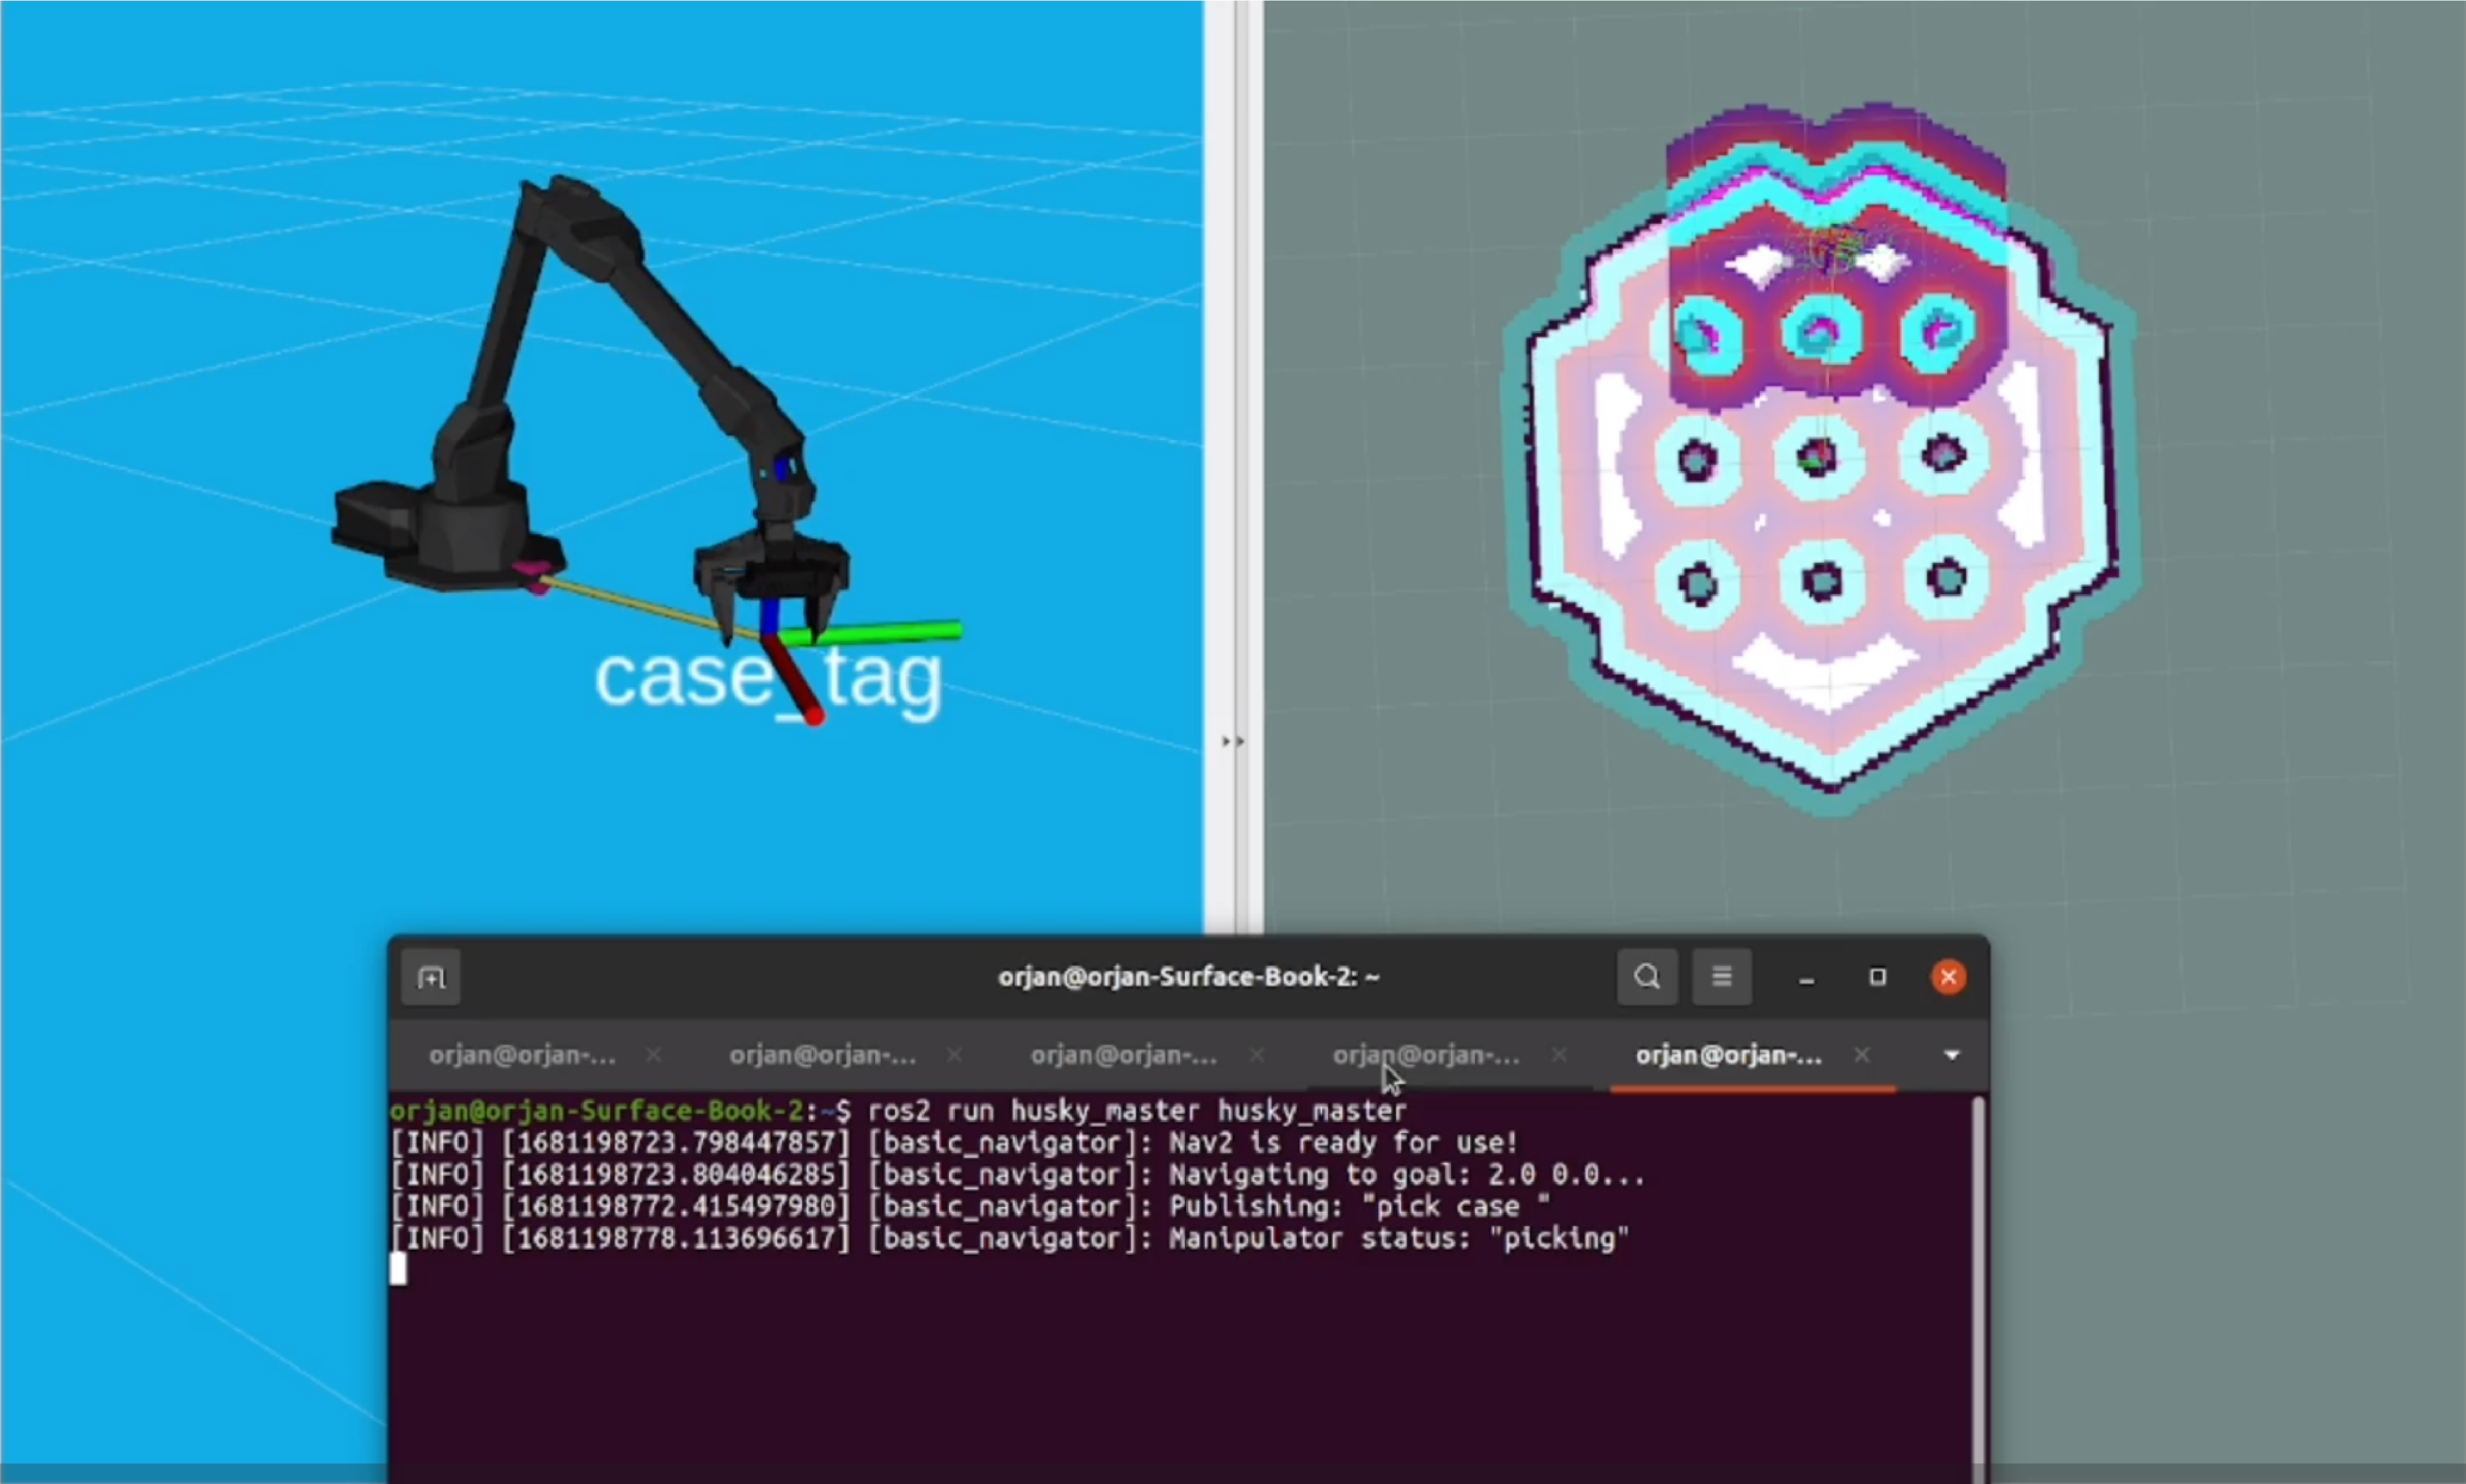
\includegraphics[width = 0.98\textwidth]{Figures/figSimTBTopLevel2.pdf}
  \caption{This figure illustrates picking operation during testing of top-level system on TurtleBot3 simulation. In this instance, the TurtleBot has reached the pick location and the manipulator is about to move its gripper down to the coordinate frame for picking. Relevant command and feedback between the Husky Master node and Pick and Place node can be seen in the terminal.}
  \label{fig:R:WA:simTBTopLevel2}
\end{figure}





%aj \section{experiment}
% write about different environment where experiment is done

% \subsection{indoor environment}

% \subsection{ware house environment}

% \section{Results}
% write that algorithms in ch 3.. was implemented to get the results with accuracy and precision, error ...

% KPI for each of functionality - show that it could navigate without collision, localize and estimate the pose of object with error xxx, pick it and place it at predefined location with error xxx

% \section{Pick and Place}



% \section{Autonomous Navigation}
% Bad kinematic design on Husky

% \section{Tag Detection}
% Worked like a charm

% \section{Pick and Place}
% Small and weak manipulator

% \section{Husky Master}
%  Unpolished Algorithm

%  \section{Husky Pick and Place}
%  Unpolished algorithm
%  Not general
%  not ideal launch file
 
%  Two methods for picking were discussed. Both of these places restrictions on the pose/shape of the objects t be picked. One method of picking bases itself on picking the objects from the side. That is, the manipulator moves in from the side of the object when gripping it. This 

%  \section{Scene Geometry Publisher}
%  Not ideal launch file
%  General design, but not general launch

 %Conclusion and Discussion